\documentclass[12pt, a4paper, oneside]{Thesis} % Paper size, default font size and one-sided paper
\usepackage{wrapfig}
\usepackage{lscape}
\usepackage{rotating}
\usepackage{graphicx}
\usepackage{caption}
\usepackage{amsmath}


\usepackage{lineno,hyperref}
\modulolinenumbers[5]


\usepackage{amssymb}
\usepackage{graphicx}
\usepackage{array}
\usepackage{float}
\usepackage{placeins}
\usepackage{stackengine}
\usepackage{url}
\usepackage{numprint}
\usepackage{caption}
 	 	
\usepackage{booktabs}  
\usepackage{siunitx}
%\usepackage[showframe=false]{geometry}
\usepackage{subfigure}
\usepackage{amsmath}

\nprounddigits{3}
\newcolumntype{P}[1]{>{\centering\arraybackslash}p{#1}}
\newcolumntype{M}[1]{>{\centering\arraybackslash}m{#1}}

\setstackEOL{\#}
\setstackgap{L}{12pt}

% Mychapter : No "Chapter X" at start, No numbering in TOC
\newcommand{\mychapter}[2]{
    \setcounter{chapter}{#1}
    \setcounter{section}{0}
    \chapter*{#2}
    \addcontentsline{toc}{chapter}{#2}
    \lhead{\emph{#2}}
}

% Enables row styling (ex. make whole row bold texted)
\newcolumntype{`}{>{\global\let\currentrowstyle\relax}}
\newcolumntype{^}{>{\currentrowstyle}}
\newcommand{\rowstyle}[1]
{\gdef\currentrowstyle{#1}%
  #1\ignorespaces
}

% To have continious table numbering
\usepackage{chngcntr}
\counterwithout{table}{chapter}

\usepackage{adjustbox}

%\usepackage{subcaption} %incompatible with subfig
\graphicspath{{Pictures/}} % Specifies the directory where pictures are stored
\usepackage{natbib} % Use the natbib reference package - read up on this to edit the reference style; if you want text (e.g. Smith et al., 2012) for the in-text references (instead of numbers), remove 'numbers' v

\hypersetup{urlcolor=black, colorlinks=true} % Colors hyperlinks in blue - change to black if annoyingv`	

\thesistitle{Semantic similarity in Q\&A using Deep learning techniques}
\supervisor{Professor Pawan Goyal}
\degree{Masters of Technology}
\degreemajor{Computer Science and Engineering}
\authors{Sandesh C}
\rollno{12CS30041}
\university{IIT Kharagpur}
\department{Department of Computer Science and Engineering}
\unisite{http://www.iitkgp.ac.in}
\depsite{http://www.cse.iitkgp.ac.in}
\placeshrt{Kharagpur}
\placelng{Kharagpur - 721302, India}
\datesub{April 28, 2017}
\datesig{April XX, 2017}
\semsub{Spring Semester, 2016-17}
%\keywords{Deep learning in Q\&A}
\coursecd{Master's Thesis Project }

\title{\ttitle} % Defines the thesis title - don't touch this
\begin{document}
%\makeatletter
%\renewcommand*{\NAT@nmfmt}[1]{\textsc{#1}}
%\makeatother

% prints author names as small caps


\frontmatter % Use roman page numbering style (i, ii, iii, iv...) for the pre-content pages

\setstretch{1.6} % Line spacing of 1.6 (double line spacing)

% Define the page headers using the FancyHdr package and set up for one-sided printing
\fancyhead{} % Clears all page headers and footers
\rhead{\thepage} % Sets the right side header to show the page number
\lhead{} % Clears the left side page header

%\pagestyle{fancy} % Finally, use the "fancy" page style to implement the FancyHdr headers

\newcommand{\HRule}{\rule{\linewidth}{0.5mm}} % New command to make the lines in the title page

% PDF meta-data
\hypersetup{pdftitle={\ttitle}}
\hypersetup{pdfsubject=\subjectname}
\hypersetup{pdfauthor=\authornames}
\hypersetup{pdfkeywords=\keywordnames}

%----------------------------------------------------------------------------------------
%	TITLE PAGE
%----------------------------------------------------------------------------------------
\maketitle
%\titlepg % Add a gap in the Contents, for aesthetics

\clearpage % Start a new page

%----------------------------------------------------------------------------------------
%	DECLARATION PAGE
%	Your institution may give you a different text to place here
%----------------------------------------------------------------------------------------


\Declaration% Add a gap in the Contents, for aesthetics


%----------------------------------------------------------------------------------------
%	CERTIFICATE PAGE
%----------------------------------------------------------------------------------------

\addtotoc{Certificate} % Add the "Abstract" page entry to the Contents

\certificate{\addtocontents{toc}{}} % Add a gap in the Contents, for aesthetics

\clearpage % Start a new page

%----------------------------------------------------------------------------------------
%	ABSTRACT PAGE
%----------------------------------------------------------------------------------------

\addtotoc{Abstract} % Add the "Abstract" page entry to the Contents

\abstract{\addtocontents{toc}{} % Add a gap in the Contents, for aesthetics

Community Question Answering (CQA) forums have since long been plagued with the problem of answer reranking, to automate the process of finding good comments to a question. Here in this work, we take up the problem of Question-Comment similarity with a simple approach where a question-comment pair is represented as concatenation of: distributed paragraph vector representations of question text, comment text and centroidal comment (of that question), along with various syntactic and metadata features. A multilayer perceptron is used to compute the similarity scores for such a question-commnet pair. 

Despite it's simplicity the model attains competitive results compared to the best submissions at SemEval '16 Task 3 - Community Question Answering (Subtask A).
}

\clearpage % Start a new page



%----------------------------------------------------------------------------------------
%	ACKNOWLEDGEMENTS
%----------------------------------------------------------------------------------------

\setstretch{1.3} % Reset the line-spacing to 1.3 for body text (if it has changed)

\acknowledgements{\addtocontents{toc}{}%\vspace{1em}} % Add a gap in the Contents, for aesthetics

First and foremost I would like to thank my guide, Prof. Pawan Goyal, for providing an opportunity to work on a challenging and relevant problem, that has blossomed to be a great learning experience. I also thank Prof. Pawan Goyal, for the constant support and guidance over the course of the project.

I would like to thank our faculty advisor, Prof. Rajat Subhra Chakraborty, for his continued efforts to help and enrich the academic experience our batch on vairous occasions. Also to acknowledge, the Department of Computer Science and Engineering, IIT Kharagpur, has been helpful through providing easy access to substantial resources for computation.

Finally I would like to thank my parents, family and friends for their continued belief and support through out the course of the programme.

}
\clearpage % Start a new page

%----------------------------------------------------------------------------------------
%	LIST OF CONTENTS/FIGURES/TABLES PAGES
%----------------------------------------------------------------------------------------

\pagestyle{fancy} % The page style headers have been "empty" all this time, now use the "fancy" headers as defined before to bring them back

\lhead{\emph{Contents}} % Set the left side page header to "Contents"
\tableofcontents % Write out the Table of Contents

%\lhead{\emph{List of Figures}} % Set the left side page header to "List of Figures"
%\listoffigures % Write out the List of Figures

\lhead{\emph{List of Tables}} % Set the left side page header to "List of Tables"
\listoftables % Write out the List of Tables

%----------------------------------------------------------------------------------------
%	ABBREVIATIONS
%----------------------------------------------------------------------------------------

\clearpage % Start a new page

\setstretch{1.5} % Set the line spacing to 1.5, this makes the following tables easier to read

\lhead{\emph{Abbreviations}} % Set the left side page header to "Abbreviations"
\listofsymbols{ll} % Include a list of Abbreviations (a table of two columns)
{
\textbf{CQA} & \textbf{C}ommunity \textbf{Q}uestion \textbf{A}nswering \\
\textbf{QL} & \textbf{Q}atar \textbf{L}iving \\
\textbf{SGD} & \textbf{S}tochastic \textbf{G}radient \textbf{D}escent \\
\textbf{PV} & \textbf{P}aragraph \textbf{V}ector \\
\textbf{CBOW} & \textbf{C}ontinious \textbf{B}ag-\textbf{O}f-\textbf{W}ords \\
\textbf{DM} & \textbf{D}istributed \textbf{M}emory \\
\textbf{DBOW} & \textbf{D}istributed \textbf{B}ag-\textbf{O}f-\textbf{W}ords \\
\textbf{MAP} & \textbf{M}ean \textbf{A}veraged \textbf{P}recision \\
\textbf{MRR} & \textbf{M}ean \textbf{R}eciprocal \textbf{R}ate \\
\textbf{AvgRec} & \textbf{Av}era\textbf{g}e \textbf{Rec}all \\
\textbf{P} & \textbf{P}recision \\
\textbf{R} & \textbf{R}ecall \\
\textbf{Acc} & \textbf{Acc}uraccy \\
%\textbf{Acronym} & \textbf{W}hat (it) \textbf{S}tands \textbf{F}or \\
}

%----------------------------------------------------------------------------------------
%	PHYSICAL CONSTANTS/OTHER DEFINITIONS
%----------------------------------------------------------------------------------------
%
%\clearpage % Start a new page
%
%\lhead{\emph{Physical Constants}} % Set the left side page header to "Physical Constants"
%
%\listofconstants{lrcl} % Include a list of Physical Constants (a four column table)
%{
%Speed of Light & $c$ & $=$ & $2.997\ 924\ 58\times10^{8}\ \mbox{ms}^{-\mbox{s}}$ (exact)\\
%% Constant Name & Symbol & = & Constant Value (with units) \\
%}

%----------------------------------------------------------------------------------------
%	SYMBOLS
%----------------------------------------------------------------------------------------

%\clearpage % Start a new page
%
%\lhead{\emph{Symbols}} % Set the left side page header to "Symbols"
%
%\listofnomenclature{lll} % Include a list of Symbols (a two column table)
%{
%$D^{el}$ & elasticity tensor \\
%$\sigma$ & stress tensor \\
%$ \varepsilon $ & strain tensor \\
%% Symbol & Name & Unit \\
%
%}

%----------------------------------------------------------------------------------------
%	DEDICATION
%----------------------------------------------------------------------------------------
%
%\setstretch{1.3} % Return the line spacing back to 1.3
%
%\pagestyle{empty} % Page style needs to be empty for this page
%
%\dedicatory{For/Dedicated to/To my\ldots} % Dedication text
%
%\addtocontents{toc}{\vspace{2em}} % Add a gap in the Contents, for aesthetics

%----------------------------------------------------------------------------------------
%	THESIS CONTENT - CHAPTERS
%----------------------------------------------------------------------------------------

\mainmatter % Begin numeric (1,2,3...) page numbering

\pagestyle{fancy} % Return the page headers back to the "fancy" style

% Include the chapters of the thesis as separate files from the Chapters folder
% Uncomment the lines as you write the chapters

%----------------------------------------------------------------------------------------
%	INTRODUCTION
%----------------------------------------------------------------------------------------

\mychapter{1}{Introduction}

\section{Introduction}

CQA forums such as Stack Overflow\footnote{https://stackoverflow.com/} and Qatar Living\footnote{http://www.qatarliving.com/}, are gaining popularity online. These forums are seldom moderated, quite open, and thus they typically have little restrictions, if any, on who can post and who can answer a question. On the positive side, this means that one can freely ask any question and can then expect some good, honest comments. On the negative side, it takes effort to go through all possible comments and to make sense of them. For example, it is not unusual for a question to have hundreds of comments, which makes it very time-consuming for the user to inspect and to winnow through them all. The present work is intended to automate the process of finding good comments to questions in a community-created discussion forum, by automatically ranking the existing comments.

\section{SemEval Task -- 3}

\textbf{SemEval Tasks}\footnote{http://alt.qcri.org/semeval2017/} (Semantic Evaluation) are an ongoing series of evaluations of computational semantic analysis systems. The \textbf{SemEval Task 3} in particular deals with semantic comparison for words and texts in the domain of Community Question Answering (CQA). In essence, the main CQA task can be defined as follows: \textit{“given (i) a new question and (ii) a large collection of question-comment threads created by a user community, rank the comments that are most useful for answering the new question”}.

\subsection{Subtask A -- Question-Comment Similarity}
In this project we address the CQA task by exploiting the semantic similarity in Q\&A using Deep learning techniques. In particular we focus on a single subtask under \textbf{SemEval - Task 3}, namely the \textbf{Subtask A}. \\ \\
\textbf{Subtask A} \textit{Given a question from a question-comment thread, rank the comments as per their relevance (similarity) with respect to the question}.

\section{Thesis Organization}
The thesis is further organized as follows: \hyperref[chap:lit-survery]{Chapter 2} addresses the recent works pertaining to the task of finding question-comment similarity, and also sheds light on a few such works that use Deep Learning methodologies to solve this problem; \hyperref[chap:approach]{Chapter 3} then provides a detailed explanation of the multilayer perceptron based prediction model approach adopted in our work, using distributed document representations and various syntactic, metadata features. Finally, \hyperref[chap:exp]{Chapter 4} tabulates the results obtained with our approach on SemEval '16 Task 3 - Subtask A dataset, which we shall see are competitive with the best results published at the same event.

%----------------------------------------------------------------------------------------
%	LITERATURE SURVEY
%----------------------------------------------------------------------------------------

\mychapter{2}{Literature Survey}
\label{chap:lit-survery}

The tasks falling under the Community Question \& Answering section of SemEval goes in the direction of passage reranking, where automatic classifiers are normally applied to pairs of questions and comment passages to derive a relative order between passages. This is in other words the task of Answer re-ranking. %For example we have works by \cite{radlinski2005query}; \cite{jeon2005finding}; \cite{shen2007using}; \cite{moschitti2007exploiting}; \cite{moschitti2008kernel}; \cite{severyn2015learning}; \cite{tymoshenko2015assessing}; \cite{tymoshenko2016convolutional}; \cite{surdeanu2008learning}.

In recent years, many advanced models have been developed for automating answer selection, producing a large body of work. For instance, \cite{wang2007jeopardy} proposed a probabilistic quasi synchronous grammar to learn syntactic transformations from the question to the candidate answers; \cite{heilman2010tree} used an algorithm based on Tree Edit Distance (TED) to learn tree transformations in pairs; \cite{wang2010probabilistic} developed a probabilistic model to learn tree-edit operations on dependency parse trees; and \cite{yao2013answer} applied linear chain CRFs with features derived from TED to automatically learn associations between questions and candidate answers. One interesting aspect of the above research is the need for syntactic structures; this is also corroborated in [\cite{severyn2012structural}; \cite{severyn2013automatic}]. Note that answer selection can use models for textual entailment, semantic similarity, and for natural language inference in general.

Although recently quite a few work in this domain have started to adopt Deep Learning Techniques to solve the problem of answer re-ranking. For eg. \cite{lin2015icrc} treated the answer selection task as a sequence labeling problem and proposed recurrent convolutional neural networks to recognize good comments. In a follow-up work, \cite{zhou2015answer} included long-short term memory (LSTM) units in their convolutional neural network to learn the classification sequence for the thread. In parallel, \cite{barron2015thread} exploited the dependencies between the thread comments to tackle the same task. This was done by designing features that look globally at the thread and by applying structured prediction models, such as Conditional Random Fields \cite{lafferty2001conditional}.

This research direction was further extended by \cite{joty2015global}, who used the output structure at the thread level in order to make more consistent global decisions. For this purpose, they modeled the relations between pairs of comments at any distance in the thread, and they combined the predictions of local classifiers in a graph-cut and in an ILP frameworks.

Noteably, at SemEval-2015 Task 3, \cite{shafiq2016joint} proposed two novel joint learning models that are on-line and integrate inference within the learning process. The first one jointly learns two node- and edge-level MaxEnt classifiers with stochastic gradient descent and integrates the inference step with loopy belief propagation. The second model is an instance of fully connected pairwise CRFs (FCCRF). The FCCRF model significantly outperformed all other approaches and yielded the best results on the task (SemEval-2015 Task 3). Crucial elements for its success were the global normalization and an Ising-like edge potential.

% TODO: SemEval '16

Thus influenced by the trend we shall tread in the direction of exploring Deep Learning Techniques to effectively solve the problem of finding Question - Comment similarity; building on the success of previous attempts. Note that we use the terms relevant-comment and answer interchangeably thoughout the document.


%----------------------------------------------------------------------------------------
%	APPROACH
%----------------------------------------------------------------------------------------

\mychapter{3}{Approach}
\label{chap:approach}

For this task, we adopt a neural approach to open-domain non-factoid QA developed by \cite{bogdanova2016we}, which focused on “answer re-ranking”, i.e. given a list of candidate answers to a question, order the answers according to their relevance to the question. The approach is very simple and requires no feature engineering. Question-answer pairs are represented by concatenated distributed representation vectors and a multilayer perceptron is used to compute the score for an answer (the probability of an answer being the best answer to the question). Despite its simplicity, their work achieved state-of-the-art performance on the Yahoo! Answers dataset of manner or How questions introduced by \cite{jansen2014discourse}. This improved performance was attributed to the use of paragraph vector representations instead of averaging over word vectors, and to the use of suitable data for training these representations. This project aims at improving the simplistic model proposed by \cite{bogdanova2016we} with a few enhancements to achieve state-of-art performance at the \textbf{SemEval Task 3 - Subtask A} of finding Question -- Comment similarity.

It is for this reason we use Paragraph Vectors (\cite{le2014distributed}) for quantifying the question-comment text documents. Paragraph Vector is an unsupervised framework that learns continuous distributed vector representations for pieces of texts. The texts can be of variable-length, ranging from sentences to documents. The name Paragraph Vector is to emphasize the fact that the method can be applied to variable-length pieces of texts, anything from a phrase or sentence to a large document.

\section{Learning Algorithm}
\label{section:learning-algo}

We used a simple feedforward neural network, i.e. a multilayered perceptron, to predict the best answer as performed by \cite{bogdanova2016we}. As shown in \autoref{fig:ann-arch}, the first layer of network takes the vector representation for a question-comment pair \textit{(q, c)} as input, which is a concatenation of the distributed representations \textit{q} and \textit{c} for the question and the comment respectively. Each representation is a real-valued vector of a fixed dimensionality \textit{d}, which is a parameter to be tuned. The input layer is concatenated with another \textit{d} dimensional vector, namely the centroidal comment, which is centroid of the distributed representation of all comments to the question q (\autoref{subsection:centroidal-comment}). This is further concatenated with another set of features generated from the pair (q, c) as described in \autoref{subsection:feature-set}. The latter two enhancements is the reason our approach shall improve upon the performance achieved by \cite{bogdanova2016we}.

\begin{figure}[t!]
  \centering
  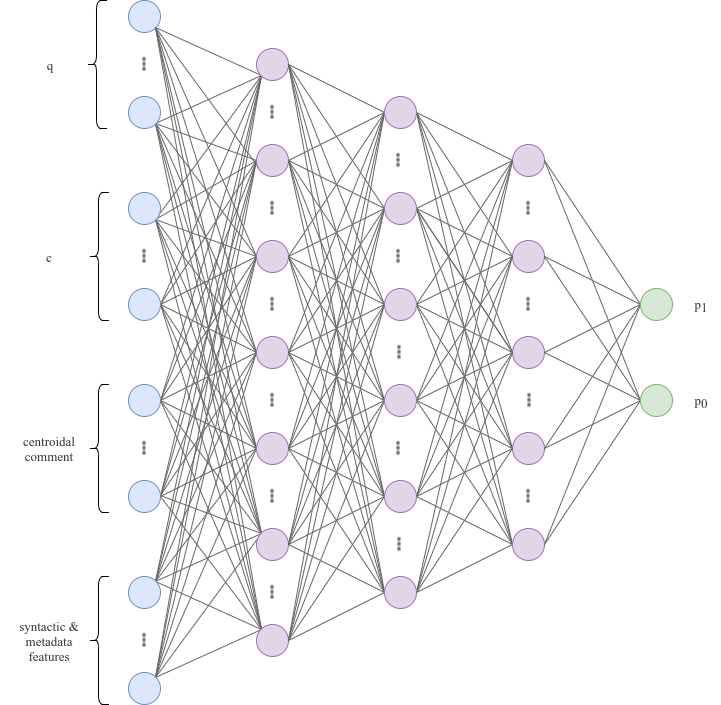
\includegraphics[keepaspectratio, width=0.8\textwidth]{./Pictures/ann-arch.png}
  \caption{Architecture of proposed Feedforward Neural Network}
  \label{fig:ann-arch}
\end{figure}

This layer is then followed by one or more hidden layers, the number of layers and units in each of these layers are also parameters to be experimentally tuned. We consider the activation function as well to be a parameter to be tuned by exprimentation. Finally, a softmax layer is used to compute the output probability p, i.e. the probabilities p1 and p2 of the negative (i.e. not best answer) and positive (i.e. best answer) classes respectively. For each question, all its user-generated comments are ranked according to their probability of being the best answer, as predicted by the network.

Given a question-comment pair (q, c), the possible values for the ground-truth label are 1 (best answer) and 0 (not a best answer). The network is trained by minimizing the L2-regularized cross-entropy loss function between the ground-truth labels and the network predictions on the training set. We use either stochastic gradient descent (SGD) or Adam solver and early stopping to minimize the loss over the training set.

\section{Document Representations}

This approach requires question-comment pairs to be represented as a fixed-size vector. We experimentally evaluate the Paragraph Vector model (PV) proposed by \cite{le2014distributed}. The PV is an extension of the widely used continuous bag-of-words (CBOW) and skip-gram word embedding models, known as word2vec. However, in contrast to CBOW and skip-gram models that only learn word embeddings, the PV is able to learn representations for pieces of text of arbitrary length, e.g. sentences, paragraphs or documents. The types of PV include (1) the distributed memory (DM) model, that predicts the next word in a text window using the concatenation of the word vectors of previous words and the paragraph vector; (2) the distributed bag-of-words (DBOW) model, that – similar to the skip-gram model – predicts words (in a small window) randomly sampled from the paragraph, given the paragraph vector. We experiment with both DM and DBOW models. \autoref{fig:pv-dm} and \autoref{fig:pv-dbow} provide an illustration for these paragraph vector models. Also, note that we shall use the terms paragraph vector (PV) and document vector/representation interchangeably.

\begin{figure}[t!]
  \centering
  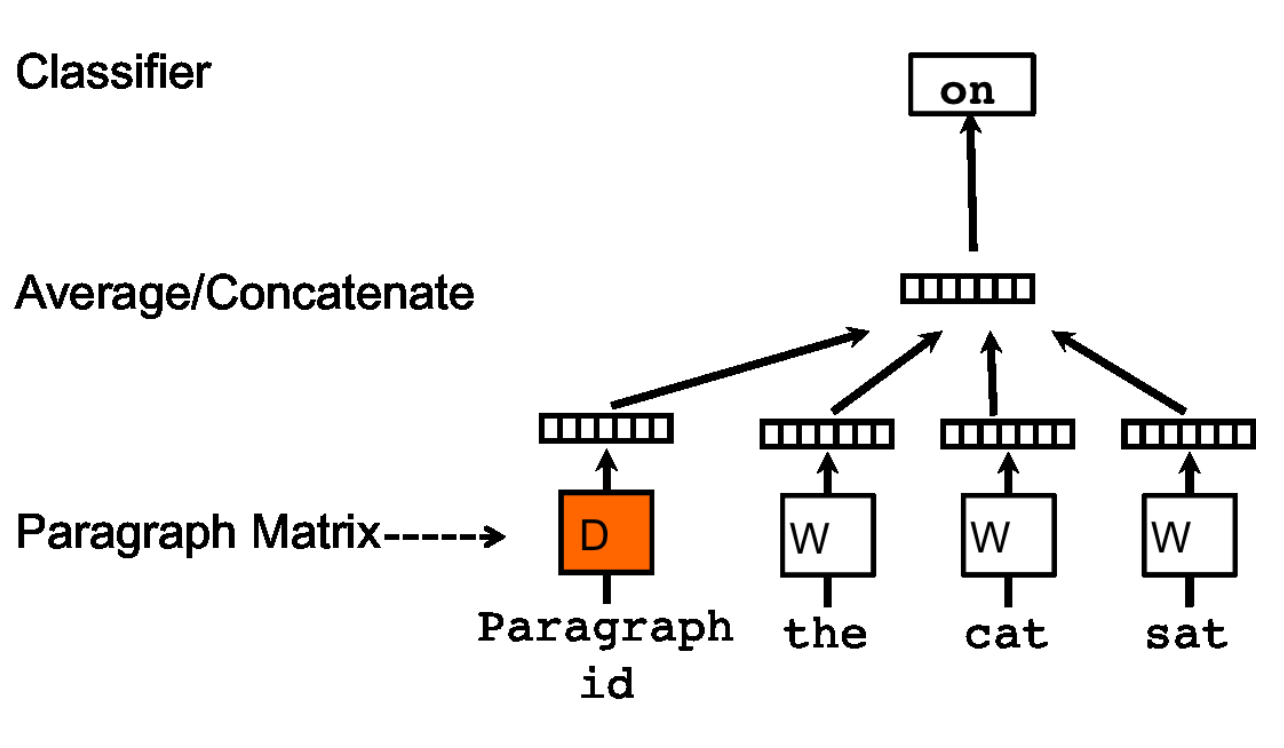
\includegraphics[keepaspectratio, width=0.8\textwidth]{./Pictures/pv-dm.png}
  \caption{Distributed Memory (DM) framework for learning paragraph vector. In this model, the concatenation or average of word vectors with a context of few words is used to predict the next word. The paragraph vector represents the missing information from the current context and can act as a memory of the topic of the paragraph.}
  \label{fig:pv-dm}
\end{figure}

\begin{figure}[t!]
  \centering
  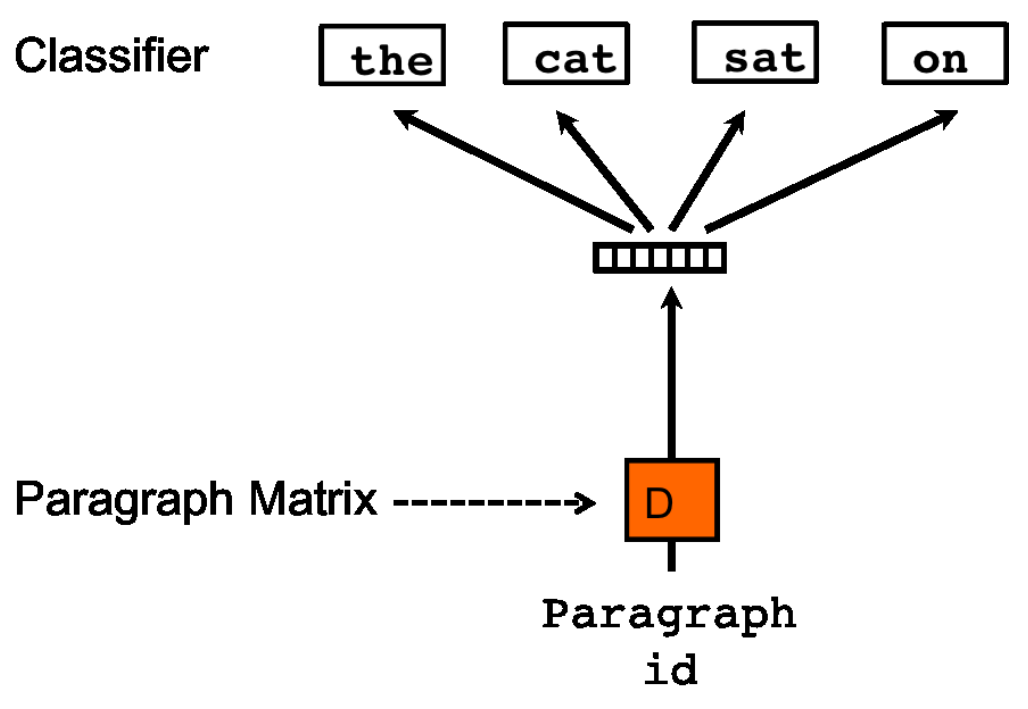
\includegraphics[keepaspectratio, width=0.8\textwidth]{./Pictures/pv-dbow.png}
  \caption{Distributed Bag of Words (DBOW) version of paragraph vectors. The paragraph vector is trained to predict the words in a small window}
  \label{fig:pv-dbow}
\end{figure}

\section{Feature Set}
\label{subsection:feature-set}

Apart from paragraph vectors of the Question (q) and Comment (c) that the feedforward network takes as input, we describe below the surplus features incorporated in our model:

\subsection{Centroidal Comment}
\label{subsection:centroidal-comment}

Inorder to rank the comments, it is only intuition that we must use the information in other comment texts to accurately provide relative relevance scores, which in turn reflects the rank, for comment texts. It is for this reason we introduced the centroidal comment, denoted as $avg\_com_q$, computed as:
\[ avg\_com_q = \frac{\sum\limits_{c \in q} c}{||\sum\limits_{c \in q} c||} \tag{1} \label{equation:1} \]

\subsection{Syntactic and Metadata Features}
\label{subsection:extra-feat}
We used several semantic vector similarity and metadata feature groups as mentioned in \cite{mihaylov2016semanticz}. For the ease of the reader, we shall describe the same feature groups below. 

Note that for the similarity measures mentioned below, we used cosine similarity:
\[ 1 - \frac{u.v}{||u||.||v||} \tag{2} \label{equation:2} \]

\textbf{Semantic Word Embeddings.} We used semantic word embeddings obtained from Word2Vec models trained on the unannotated data set from QatarLiving. For each piece of text such as comment text, question body and question subject, we constructed the centroid vector from the vectors of all words in that text (excluding stopwords).
\[ centroid(w_{1...n}) = \frac{\sum\limits_{i=1}^{n} w_i}{n} \tag{3} \label{equation:3} \]
We construct centroid vectors (3) from the question text (subject + body) and the comment text to design various features as described below.

\textbf{Semantic Vector Similarities.} We used various similarity features calculated using the centroid word vectors on the question text (subject + body) and on the comment text, as well as on parts thereof:

\textbf{Question to Answer similarity.} We assume that a relevant answer should have a centroid vector that is close to that for the question. We used the question text to comment text vector similarities.

\textbf{Maximized similarity.} We ranked each word in the comment text to the question text centroid vector according to their similarity and we took the average similarity of the top N words. We took the top 1, 2, 3, 4 and 5 words similarities as features. The assumption here is that if the average similarity for the top N most similar words is high, then the comment might be relevant.

\textbf{Aligned similarity.} For each word in the question text, we chose the most similar word from the comment text and we took the average of all best word pair similarities as suggested in \cite{tran2015jaist}.

\textbf{Part of speech (POS) based word vector similarities.} We performed part of speech tagging using the Stanford tagger \cite{toutanova2003feature}, and we took similarities between centroid vectors of words with a specific tag from the comment text and the centroid vector of the words with a specific tag from the question text. The assumption is that some parts of speech between the question and the comment might be closer than other parts of speech.

\textbf{Word clusters (WC) similarity.} We clustered the word vectors from the Word2Vec vocabulary in 1,000 clusters using K-Means clustering. We then calculated the cluster similarity between the question body word clusters and the answer text word clusters. For all experiments, we used clusters obtained from the Word2Vec model trained on QatarLiving forums with vector size of 100, window size 10.

\textbf{LDA topic similarity.} We performed topic clustering using Latent Dirichlet Allocation (LDA) as implemented in the gensim toolkit \cite{rehurek2010software} on Train1 + Train2 + Dev questions and comments. We built topic models with 100 topics. For each word in the question text and for the comment text, we built a bag-of-topics with corresponding distribution, and calculated similarity. The assumption here is that if the question and the comment share similar topics, they are more likely to be relevant to each other

\textbf{Paragraph Vector similarities.} The similarity among the distributed vector representations of question text (\textit{q}), answer text (\textit{a}) and the centroidal answer ($avg\_com_q$), taken two at a time are also included.

\textbf{Metadata.} In addition to the semantic features described above, we also used some common sense metadata features:

\textbf{Answer contains a question mark.} If the comment has an question mark, it may be another question, which might indicate a bad answer.

\textbf{Answer length.} Assumption here is that longer answers could bring useful details.

\textbf{Question length.} If the question is longer, it may be more clear, which may help users give a more relevant answer.

\textbf{Question to comment length.} If the question is long and the answer is short, it may be less relevant.

\textbf{The answer’s author is the same as the corresponding question’s author.} If the answer is posted by the same user who posted the question and it is relevant, why has he/she asked the question in the first place?

\textbf{Answer rank in the thread.} Earlier answers could be posted by users who visit the forum more often, and they may have read more similar questions and answers. Moreover, discussion in the forum tends to diverge from the question over time.

\textbf{Question category.} We took the category of the question as a sparse binary feature vector (a feature with a value of 1 appears if question is in the category). The assumption here is that the question-comment relevance might depend on the category of the question.

\textbf{Comments by the same User.} The number of comments by the author of a given comment to the same question and the order of the comments (first, second, ...) is also included as a feature. If the author produced an incomplete answer in the first attempt, he/she might be obliged to produce another comment subsequently.

\textbf{Time difference between Question and Comment posting.} Immediate comments could reflect incomplete answers to longer questions, while comments posted after substantial time might reflect well-thought answers.

%----------------------------------------------------------------------------------------
%	EXPERIMENTS
%----------------------------------------------------------------------------------------

\mychapter{4}{Experiments}
\label{chap:exp}

\section{Data}

Though \cite{bogdanova2016we} experiments with the \textit{Yahoo! Answers dataset}\footnote{http://webscope.sandbox.yahoo.com/}, we have used the data provided as a part of the popular \textbf{SemEval Task 3} for \textbf{Subtask A} (\cite{nakov-EtAl:2016:SemEval}). \autoref{table:data} contains the statistics about the forementioned dataset. This dataset contains about 42K (q, c) pairs to learn from; spreading over about 5.4K questions. We shall refer to this data as the CQA-QL corpus in future. Further we also use a large unannotated dataset, released by the same source, from Qatar Living with 189,941 questions and 1,894,456 comments, which is used for unsupervised learning/training domain-specific word/document embeddings. \\

\setcounter{table}{0}
\begin{table}[!htbp]
\centering
\begin{adjustbox}{max width=\textwidth,center}
\begin{tabular}{`l^r^r^r^r^r^r}
\rowstyle{\bfseries}
Category 			&	Train 		&	Train		&	Train+Dev+Test		&	Dev		&	Test		&	Total	\\
\rowstyle{\bfseries}
					&	(Part-I)		&	(Part-II)	&	(from SemEval 2015)	&			&			&			\\
\\\hline\\
\rowstyle{\bfseries}
Questions			&	1,411		&	379			&	2,480+291+319		&	244		&	327		&	5,451	\\\\
\rowstyle{\bfseries}
Comments				&	14,110		&	3,790		&	14,893+1,529+1,876	&	2,440	&	3,270	&	41,908	\\
\rowstyle{\itshape}
-Good				&	5,287		&	1,364		&	7,418+813+946		&	818		&	1,329	&	17,975	\\
\rowstyle{\itshape}
-Bad					&	6,362		&	1,777		&	5,971+544+774		&	1,209	&	1,485	&	18,122	\\
\rowstyle{\itshape}
-Potentially			&	2,461		&	649			&	1,504+172+156		&	413		&	456		&	5,811	\\
\hline
\end{tabular}
\end{adjustbox}
\caption{Statistics on English CQA-QL corpus \\from SemEval-2017 Task 3 (Subtask A)}
\label{table:data}
\end{table}

\section{Experimental Setup}

We use the gensim\footnote{https://radimrehurek.com/gensim/models/doc2vec.html} implementation of DM and DBOW paragraph vector models. The data for training the unsupervised \textit{doc2vec} model (PV model) is the forementioned large unannotated dataset from Qatar Living forums. Each paragraph (q or c) was converted to lowercase, tokenized by space character and cleaned of stop words before training \textit{doc2vec} models. The parameters of training these models being the window size (maximum distance between the predicted word and context words used for prediction within a document) and number of epochs of training, were cross-validated to give low errors on the training dataset. We further use normalized versions of the document vector representations thus generated, to be fed as inputs to the feedforward neural network described in \autoref{section:learning-algo}. \\ \\
For the implementation of the feedforward neural network as described in \autoref{section:learning-algo}, we shall use the popular python library \textit{scikit-learn\footnote{http://scikit-learn.org/stable/index.html}}'s \textit{MLPClassifier}\footnote{http://scikit-learn.org/stable/modules/generated/sklearn.neural\_network.MLPClassifier.html}.

\section{Results}

\subsection{Document Vector Representations}

For training each question/comment text was treated as a document/paragraph and assigned a label, which can be used as a key to retrieve the document vector. Furthermore post training the doc2vec model is able to infer a document vector for any new question/comment text whose vocabulary is from the original corpus. The errors post training is computed as averaged squared error over all question/comment text, by computing squared error between the document vector learnt by the model corresponding to the text’s label and the document vector inferred from the question/comment text. The squared errors are computed for normalizeddocument vectors. For comparison purposes squared error between any two random (normalized) document vector is tabulated beside these errors (averaged over as many iterations as the number of question/comment text). Experiments show that 100-dimensional PV trained over the $\sim$2.3M samples from the unannotated QL corpus, gives sufficiently low errors post normalization. Further more, PV-DBOW proves to outperform the PV-DM representations as seen in \autoref{table:pv-train-best}. It contains few of the best results has rows sorted by the value of \textit{column \lq{Ratio}\rq}, as it is the indicator of how good the representation is. The complete list of experiments are tabulated under \autoref{table:pv-train-full} in \autoref{appendix:A}.

%\setcounter{table}{1}
\begin{table}[!htbp]
\centering
\begin{adjustbox}{max width=\textwidth,center}
\begin{tabular}{`c^c^c^c^c^c^c^c}
\rowstyle{\bfseries}
Category 			&	Window 	&	Epochs	&	Normalized	&	Norm. Sq. Error	&	Ratio\\
\rowstyle{\bfseries}
					&	Size		&			&	Sq. Error (A)	&	(Random)	(B)		&	(B/A)\\
\\\hline\\
PV-DBOW & 10 & 5 & 0.14 & 0.80 & 5.89 \\
PV-DBOW & 10 & 10 & 0.14 & 0.83 & 5.84 \\
PV-DM & 10 & 5 & 0.21 & 0.99 & 4.67 \\
PV-DM & 15 & 10 & 0.22 & 0.98 & 4.47 \\
\hline
\end{tabular}
\end{adjustbox}
\caption{Training document vector representations PV-DM and PV-DBOW -- Best results}
\label{table:pv-train-best}
\end{table}

To decide upon the dimension of the paragraph vectors we conduct similar experiments by testing on PV-DBOW document vectors of size 100 and 200. The best results tabulated in \autoref{table:pv-dimen-best}, show that 100 dimensional paragraph vectors prove to be a better choice owing to having both: higher accuracy and low computational complexity. The complete list of experiments are tabulated under \autoref{table:pv-dimen-full} in \autoref{appendix:A}.

\begin{table}[!htbp]
\centering
\begin{adjustbox}{max width=\textwidth,center}
\begin{tabular}{`c^c^c^c^c^c^c^c}
\rowstyle{\bfseries}
Dimension 			&	Window 	&	Epochs	&	Normalized	&	Norm. Sq. Error	&	Ratio\\
\rowstyle{\bfseries}
					&	Size		&			&	Sq. Error (A)	&	(Random)	(B)		&	(B/A)\\
\\\hline\\
100 & 10 & 5 & 0.14 & 0.80 & 5.89 \\
100 & 10 & 10 & 0.14 & 0.83 & 5.84 \\
200 & 10 & 10 & 0.15 & 0.84 & 5.65 \\
200 & 10 & 5 & 0.15 & 0.82 & 5.47 \\
\hline
\end{tabular}
\end{adjustbox}
\caption{Training PV-DBOW document vectors of sizes 100 and 200 -- Best results}
\label{table:pv-dimen-best}
\end{table}

\subsection{SemEval Task 3 -- Subtask A}

The training data comprises of 38,638 comments spanning over 5,124 questions. The neural net input is a tuple of the form $(q, c, avg\_ans_q, ft_{(q,c)})$, where, \\
\hspace*{1cm}$avg\_com_q$ is (normalized) average over the PV of all comments to question q \\
\hspace*{1cm}$ft_{(q,c)}$ is feature vector corresp. to the pair (q,c) as described in \autoref{subsection:feature-set}
\\\\
\textbf{SemEval Task 3} has as an official evaluation measure used to rank the participating systems, the metric of Mean Average Precision (\textit{MAP}), calculated for the ten comments a participating system has ranked highest. Further metrics such as Mean Reciprocal Rank (\textit{MRR}) and Average Recall (\textit{AvgRec}) for top-10 results; Precision (\textit{P}), Recall (\textit{R}), \textit{F\textsubscript{1}} (with respect to the Good/Relevant class) and Accuracy (\textit{Acc}) are also reported.

\subsubsection{Preliminary experiments with (q, c) inputs}

Intially experiments were conducted with only (q, c) pair as input to the neural nets. The nets were trained using multiple solvers, activation functions, hidden layer configurations. The best performance for each parameter configuration is as tabulated in \autoref{table:ann-stage-1-best}, while the complete results are tabulated in \autoref{appendix:B}.

%\setcounter{table}{2}
\begin{table}[!htbp]
\centering
\begin{adjustbox}{max width=\textwidth,center}
\begin{tabular}{`c^c^c^c^c^c^c^c^c^c}
\rowstyle{\bfseries}
Category & Solver & Activation & MAP & AvgRec & MRR & P & R & F\textsubscript{1} & Acc \\
\\\hline\\
PV-DBOW & Adam & logistic & \textbf{70.49} & 82.92 & 77.62 & 66.01 & 55.08 & 60.05 & 70.21 \\
PV-DBOW & SGD & relu & 70.19 & 82.51 & 77.16 & 63.27 & 59.37 & 61.26 & 69.48 \\
PV-DBOW & SGD & logistic & 70.18 & 82.42 & 77.32 & 64.12 & 58.77 & 61.33 & 69.88 \\
PV-DBOW & SGD & tanh & 70.09 & 82.45 & 76.62 & 63.39 & 59.14 & 61.19 & 69.51 \\
PV-DBOW & Adam & relu & 69.93 & 81.06 & 76.94 & 59.98 & 57.41 & 58.67 & 67.13 \\
PV-DBOW & Adam & tanh & 69.80 & 82.31 & 76.35 & 63.86 & 55.46 & 59.36 & 69.14 \\
PV-DM & SGD & relu & 65.78 & 78.55 & 74.58 & 57.93 & 53.57 & 55.67 & 65.32 \\
\hline
\end{tabular}
\end{adjustbox}
\caption{Preliminary experiments using only $(q, c)$ inputs -- Best results}
\label{table:ann-stage-1-best}
\end{table}

PV-DBOW clearly outperforms PV-DM representations in these preliminary runs. Building on this, further experiments where conducted using only the PV-DBOW representations.

\subsubsection{Improvement with inclusion of Centroidal comment}

As described in \autoref{subsection:centroidal-comment}, additionally, to capture the relative goodness of an comment with respect to other comments to the same question, $avg\_com_q$ (normalized post averaging over the PV of all comments to question q) was fed as an input to the neural net. The best results for these experiments are tabulated in \autoref{table:ann-stage-2-best}. Complete results are tabulated under \autoref{appendix:C}.

\begin{table}[!htbp]
\centering
\begin{adjustbox}{max width=\textwidth,center}
\begin{tabular}{`c^c^c^c^c^c^c^c^c^c}
\rowstyle{\bfseries}
Category & Solver & Activation & MAP & AvgRec & MRR & P & R & F\textsubscript{1} & Acc \\
\\\hline\\
PV-DBOW & SGD & relu & \textbf{73.06} & 84.16 & 79.61 & 66.07 & 57.86 & 61.69 & 70.8 \\
PV-DBOW & SGD & tanh & 71.88 & 83.43 & 79.11 & 66.84 & 56.58 & 61.29 & 70.95 \\
PV-DBOW & SGD & logistic & 71.79 & 83.46 & 79.13 & 66.52 & 55.3 & 60.39 & 70.52 \\
PV-DBOW & Adam & logistic & 71.77 & 83.42 & 78.96 & 66.35 & 57.26 & 61.47 & 70.83 \\
PV-DBOW & Adam & tanh & 71.69 & 83.39 & 78.64 & 65.5 & 57.71 & 61.36 & 70.46 \\
PV-DBOW & Adam & relu & 71.61 & 82.63 & 79.45 & 62.98 & 60.05 & 61.48 & 69.42 \\
\hline
\end{tabular}
\end{adjustbox}
\caption{Experiments using $(q, c, avg\_com_q)$ inputs -- Best results}
\label{table:ann-stage-2-best}
\end{table}

Clearly there is a significant improvement in MAP scores after inclusion of the centroidal comment for each question as an input feature. Further experiments thus is done inclusive of $avg\_com_q$ in the input tuple.

\subsubsection{Further improvement with Syntactic and Metadata Features}

Finally, we experimented by including a few more features as described in \autoref{subsection:extra-feat}; which includes various thread level metadata features, and features that capture syntactic similarities between the question and comment text. The best results are tabulated in \autoref{table:ann-stage-3-best}. Complete results are tabulated under \autoref{appendix:D}. Further, we excluded the \textit{ADAM} solver from parameters, as \textit{SGD} performs significantly better on all runs (can be seen from \autoref{table:ann-stage-2-best} as well).

\begin{table}[!htbp]
\centering
\begin{adjustbox}{max width=\textwidth,center}
\begin{tabular}{`c^c^c^c^c^c^c^c^c^c}
\rowstyle{\bfseries}
Category & Solver & Activation & MAP & AvgRec & MRR & P & R & F\textsubscript{1} & Acc \\
\\\hline\\
PV-DBOW & SGD & tanh & \textbf{77.74} & 88.2 & 85.58 & 70.81 & 63.51 & 66.96 & 74.53 \\
PV-DBOW & SGD & relu & 77.43 & 87.96 & 84.81 & 70.57 & 62.6 & 66.35 & 74.19 \\
PV-DBOW & SGD & logistic & 77.26 & 87.87 & 85.51 & 71.49 & 63.58 & 67.3 & 74.89 \\
\hline
\end{tabular}
\end{adjustbox}
\caption{Experiments using $(q, c, avg\_com_q, ft_{(q,c)})$ inputs -- Best results}
\label{table:ann-stage-3-best}
\end{table}

\subsubsection{Analysis with $(q, c, ft_{(q,c)})$ inputs}

To get more insight into the contribution of each set of features, we remove the $avg\_com_q$ features and test the model. The best results are tabulated in \autoref{table:ann-stage-2half-best}, while the complete results can be found in \autoref{appendix:E}.

\begin{table}[!htbp]
\centering
\begin{adjustbox}{max width=\textwidth,center}
\begin{tabular}{`c^c^c^c^c^c^c^c^c^c}
\rowstyle{\bfseries}
Category & Solver & Activation & MAP & AvgRec & MRR & P & R & F\textsubscript{1} & Acc \\
\\\hline\\
PV-DBOW & SGD & logistic & \textbf{77.22} & 87.44 & 84.67 & 69.62 & 62.75 & 66.01 & 73.73 \\
PV-DBOW & SGD & tanh & 77.14 & 87.44 & 84.65 & 69.31 & 63.21 & 66.12 & 73.67 \\
PV-DBOW & SGD & relu & 77.03 & 87.39 & 84.8 & 70.32 & 62.75 & 66.32 & 74.10 \\
\hline
\end{tabular}
\end{adjustbox}
\caption{Experiments using $(q, c, ft_{(q,c)})$ inputs -- Best results}
\label{table:ann-stage-2half-best}
\end{table}

%----------------------------------------------------------------------------------------
%	CONCLUSIONS
%----------------------------------------------------------------------------------------

\addtocontents{toc}{\vspace{2em}} % Add a gap in the Contents, for aesthetics

\mychapter{5}{Conclusions}


%----------------------------------------------------------------------------------------
%	THESIS CONTENT - APPENDICES
%----------------------------------------------------------------------------------------

\addtocontents{toc}{\vspace{2em}} % Add a gap in the Contents, for aesthetics

\appendix % Cue to tell LaTeX that the following 'chapters' are Appendices

% Include the appendices of the thesis as separate files from the Appendices folder
% Uncomment the lines as you write the Appendices

\chapter{Training PV-DM and PV-DBOW}
\lhead{\emph{Training PV-DM and PV-DBOW}}
\label{appendix:A}

%\setcounter{table}{5}
\begin{table}[!htbp]
\centering
\begin{adjustbox}{max width=\textwidth,center}
\begin{tabular}{`c^c^c^c^c^c^c^c}
\rowstyle{\bfseries}
Category 			&	Window 	&	Epochs	&	Squared	&	Normalized	&	Sq. Error	&	Norm. Sq. Error	&	Ratio\\
\rowstyle{\bfseries}
					&	Size		&			&	Error	&	Sq. Error (A)	&	(Random)		&	(Random)	(B)		&	(B/A)\\
\\\hline\\
PV-DBOW & 10 & 5 & 10.791 & 0.118 & 0.560 & 0.799 & 6.738 \\
PV-DBOW & 10 & 10 & 13.159 & 0.124 & 0.606 & 0.821 & 6.614 \\
PV-DBOW & 15 & 5 & 10.790 & 0.127 & 0.564 & 0.796 & 6.263 \\
PV-DBOW & 15 & 10 & 13.077 & 0.132 & 0.607 & 0.818 & 6.193 \\
PV-DBOW & 20 & 5 & 10.749 & 0.134 & 0.569 & 0.794 & 5.910 \\
PV-DBOW & 20 & 10 & 12.932 & 0.140 & 0.611 & 0.816 & 5.822 \\
PV-DM & 10 & 5 & 0.664 & 0.211 & 0.985 & 0.987 & 4.671 \\
PV-DM & 15 & 10 & 0.929 & 0.219 & 0.981 & 0.983 & 4.472 \\
PV-DM & 15 & 5 & 0.670 & 0.229 & 0.984 & 0.984 & 4.291 \\
PV-DM & 20 & 10 & 0.830 & 0.229 & 0.982 & 0.982 & 4.284 \\
PV-DM & 25 & 10 & 0.780 & 0.235 & 0.983 & 0.982 & 4.168 \\
PV-DM & 20 & 5 & 0.706 & 0.239 & 0.984 & 0.981 & 4.092 \\
PV-DM & 15 & 20 & 1.597 & 0.241 & 0.970 & 0.976 & 4.034 \\
PV-DM & 25 & 5 & 0.735 & 0.248 & 0.984 & 0.980 & 3.951 \\
PV-DM & 20 & 20 & 1.434 & 0.247 & 0.974 & 0.977 & 3.947 \\
PV-DM & 25 & 20 & 1.339 & 0.251 & 0.976 & 0.978 & 3.890 \\
PV-DM & 15 & 30 & 2.062 & 0.261 & 0.954 & 0.963 & 3.687 \\
PV-DM & 20 & 30 & 1.867 & 0.266 & 0.962 & 0.968 & 3.637 \\
PV-DM & 25 & 30 & 1.741 & 0.270 & 0.966 & 0.971 & 3.595 \\
PV-DM & 10 & 1 & 0.964 & 0.333 & 0.988 & 0.979 & 2.936 \\
PV-DM & 15 & 1 & 0.975 & 0.357 & 0.988 & 0.971 & 2.717 \\
PV-DM & 20 & 1 & 0.979 & 0.374 & 0.988 & 0.969 & 2.592 \\
PV-DM & 25 & 1 & 0.981 & 0.384 & 0.988 & 0.967 & 2.515 \\
\hline
\end{tabular}
\end{adjustbox}
\caption{Training document vector representations PV-DM and PV-DBOW -- All results}
\label{table:pv-train-full}
\end{table}
\chapter{Preliminary experiments}
\lhead{\emph{Preliminary experiments -- only (q, c) inputs}}
\label{appendix:B}

%\setcounter{table}{6}
\begin{table}[!htbp]
\centering
\begin{adjustbox}{max width=\textwidth,center}
\begin{tabular}{`c^c^c^c^c^c^c^c^c^c^c^c}
\rowstyle{\bfseries}
Category & Solver & Activation & Hidden Layer & MAP & AvgRec & MRR & P & R & F\textsubscript{1} & Acc \\
\\\hline\\
PV-DBOW & Adam & logistic & [ 500, 250, - ] & 0.7049 & 0.8292 & 77.62 & 0.6601 & 0.5508 & 0.6005 & 0.7021 \\
PV-DBOW & SGD & relu & [ 100, -, - ] & 0.7019 & 0.8251 & 77.16 & 0.6327 & 0.5937 & 0.6126 & 0.6948 \\
PV-DBOW & SGD & logistic & [ 50, -, - ] & 0.7018 & 0.8242 & 77.32 & 0.6412 & 0.5877 & 0.6133 & 0.6988 \\
PV-DBOW & SGD & logistic & [ 100, -, - ] & 0.7013 & 0.8242 & 77.23 & 0.6353 & 0.5884 & 0.6109 & 0.6954 \\
PV-DBOW & SGD & tanh & [ 500, 100, 100 ] & 0.7009 & 0.8245 & 76.62 & 0.6339 & 0.5914 & 0.6119 & 0.6951 \\
PV-DBOW & Adam & logistic & [ 50, 50, 50 ] & 0.7008 & 0.8252 & 76.8 & 0.6043 & 0.6584 & 0.6302 & 0.6859 \\
PV-DBOW & SGD & relu & [ 50, -, - ] & 0.7007 & 0.824 & 77.01 & 0.6374 & 0.5899 & 0.6127 & 0.6969 \\
PV-DBOW & SGD & tanh & [ 250, 100, - ] & 0.7007 & 0.8237 & 76.86 & 0.631 & 0.5854 & 0.6073 & 0.6924 \\
PV-DBOW & Adam & logistic & [ 100, 50, 50 ] & 0.7007 & 0.8251 & 76.89 & 0.6325 & 0.5997 & 0.6157 & 0.6957 \\
PV-DBOW & SGD & logistic & [ 250, -, - ] & 0.7006 & 0.8236 & 77.36 & 0.6396 & 0.5862 & 0.6117 & 0.6976 \\
PV-DBOW & Adam & logistic & [ 100, 100, 100 ] & 0.7006 & 0.825 & 76.9 & 0.6404 & 0.5749 & 0.6059 & 0.696 \\
PV-DBOW & SGD & logistic & [ 500, -, - ] & 0.7005 & 0.824 & 77.2 & 0.6369 & 0.5847 & 0.6097 & 0.6957 \\
PV-DBOW & SGD & tanh & [ 250, 50, 50 ] & 0.7004 & 0.8241 & 76.89 & 0.6339 & 0.5914 & 0.6119 & 0.6951 \\
PV-DBOW & Adam & logistic & [ 250, 250, 250 ] & 0.7003 & 0.8248 & 76.97 & 0.6217 & 0.6245 & 0.6231 & 0.693 \\
PV-DBOW & Adam & logistic & [ 250, 250, 50 ] & 0.7 & 0.8248 & 76.94 & 0.6205 & 0.62 & 0.6202 & 0.6914 \\
PV-DBOW & Adam & logistic & [ 500, 100, - ] & 0.6999 & 0.8244 & 76.92 & 0.6281 & 0.6087 & 0.6183 & 0.6945 \\
PV-DBOW & Adam & logistic & [ 250, 100, - ] & 0.6998 & 0.824 & 76.7 & 0.6164 & 0.6275 & 0.6219 & 0.6899 \\
PV-DBOW & Adam & logistic & [ 250, 50, - ] & 0.6998 & 0.8239 & 76.66 & 0.6194 & 0.6381 & 0.6286 & 0.6936 \\
PV-DBOW & Adam & logistic & [ 500, 50, - ] & 0.6997 & 0.8243 & 76.75 & 0.6346 & 0.605 & 0.6194 & 0.6979 \\
PV-DBOW & Adam & logistic & [ 250, 250, 100 ] & 0.6997 & 0.8243 & 76.84 & 0.6343 & 0.5899 & 0.6113 & 0.6951 \\
PV-DBOW & SGD & tanh & [ 250, 100, 50 ] & 0.6996 & 0.8235 & 76.66 & 0.6334 & 0.5877 & 0.6097 & 0.6942 \\
PV-DBOW & SGD & tanh & [ 100, 100, 50 ] & 0.6996 & 0.8237 & 76.99 & 0.637 & 0.5877 & 0.6114 & 0.6963 \\
PV-DBOW & SGD & tanh & [ 100, -, - ] & 0.6996 & 0.823 & 76.67 & 0.634 & 0.5839 & 0.6079 & 0.6939 \\
PV-DBOW & Adam & logistic & [ 500, 250, 50 ] & 0.6995 & 0.8238 & 76.69 & 0.6447 & 0.5749 & 0.6078 & 0.6985 \\
PV-DBOW & SGD & tanh & [ 500, 500, 250 ] & 0.6994 & 0.8241 & 76.76 & 0.6339 & 0.5914 & 0.6119 & 0.6951 \\
PV-DBOW & SGD & tanh & [ 500, 500, 100 ] & 0.6994 & 0.8235 & 76.89 & 0.6347 & 0.5884 & 0.6107 & 0.6951 \\
PV-DBOW & SGD & tanh & [ 500, 500, - ] & 0.6994 & 0.8238 & 76.43 & 0.6347 & 0.5884 & 0.6107 & 0.6951 \\
PV-DBOW & Adam & logistic & [ 100, 100, 50 ] & 0.6994 & 0.824 & 76.51 & 0.6406 & 0.5794 & 0.6085 & 0.6969 \\
PV-DBOW & Adam & logistic & [ 100, 50, - ] & 0.6994 & 0.8243 & 76.74 & 0.6279 & 0.6095 & 0.6186 & 0.6945 \\
PV-DBOW & Adam & relu & [ 500, 50, - ] & 0.6993 & 0.8106 & 76.94 & 0.5998 & 0.5741 & 0.5867 & 0.6713 \\
PV-DBOW & SGD & tanh & [ 500, 500, 50 ] & 0.6992 & 0.8236 & 76.5 & 0.6344 & 0.5914 & 0.6121 & 0.6954 \\
\hline
\end{tabular}
\end{adjustbox}
\caption{Preliminary experiments using only (q, c) inputs -- All results (\textit{MAP}\textgreater0.6).}
\label{table:ann-stage-1-full-1}
\end{table}

%\setcounter{table}{6}
\begin{table}[!htbp]
\centering
\begin{adjustbox}{max width=\textwidth,center}
\begin{tabular}{`c^c^c^c^c^c^c^c^c^c^c^c}
\rowstyle{\bfseries}
Category & Solver & Activation & Hidden Layer & MAP & AvgRec & MRR & P & R & F\textsubscript{1} & Acc \\
\\\hline\\
PV-DBOW & SGD & tanh & [ 250, 50, - ] & 0.6992 & 0.8225 & 76.76 & 0.633 & 0.5892 & 0.6103 & 0.6942 \\
PV-DBOW & SGD & tanh & [ 100, 100, - ] & 0.6992 & 0.8241 & 76.74 & 0.6349 & 0.5862 & 0.6095 & 0.6948 \\
PV-DBOW & Adam & logistic & [ 500, 500, 500 ] & 0.6992 & 0.8246 & 76.77 & 0.6098 & 0.6584 & 0.6331 & 0.6899 \\
PV-DBOW & Adam & logistic & [ 250, 100, 50 ] & 0.6992 & 0.8238 & 76.74 & 0.6224 & 0.6275 & 0.625 & 0.6939 \\
PV-DBOW & Adam & logistic & [ 50, 50, - ] & 0.6992 & 0.8241 & 76.87 & 0.6333 & 0.6042 & 0.6184 & 0.6969 \\
PV-DBOW & SGD & tanh & [ 50, 50, - ] & 0.699 & 0.8236 & 76.77 & 0.6373 & 0.5884 & 0.6119 & 0.6966 \\
PV-DBOW & SGD & tanh & [ 50, -, - ] & 0.699 & 0.8235 & 76.95 & 0.6407 & 0.5877 & 0.613 & 0.6985 \\
PV-DBOW & SGD & relu & [ 500, -, - ] & 0.6989 & 0.824 & 76.58 & 0.6377 & 0.5907 & 0.6133 & 0.6972 \\
PV-DBOW & SGD & tanh & [ 500, 100, - ] & 0.6989 & 0.8231 & 76.79 & 0.6338 & 0.5862 & 0.6091 & 0.6942 \\
PV-DBOW & SGD & tanh & [ 250, -, - ] & 0.6987 & 0.8238 & 76.94 & 0.6321 & 0.5869 & 0.6087 & 0.6933 \\
PV-DBOW & SGD & tanh & [ 100, 100, 100 ] & 0.6987 & 0.8235 & 76.59 & 0.6365 & 0.5877 & 0.6111 & 0.696 \\
PV-DBOW & SGD & tanh & [ 500, 100, 50 ] & 0.6986 & 0.8233 & 76.5 & 0.6365 & 0.5929 & 0.6139 & 0.6969 \\
PV-DBOW & Adam & logistic & [ 100, 100, - ] & 0.6986 & 0.8235 & 76.28 & 0.6192 & 0.6253 & 0.6222 & 0.6914 \\
PV-DBOW & SGD & relu & [ 250, -, - ] & 0.6985 & 0.824 & 76.55 & 0.6369 & 0.5899 & 0.6125 & 0.6966 \\
PV-DBOW & Adam & logistic & [ 100, -, - ] & 0.6984 & 0.8232 & 76.54 & 0.643 & 0.5666 & 0.6024 & 0.696 \\
PV-DBOW & SGD & tanh & [ 500, 250, 100 ] & 0.6983 & 0.8233 & 76.2 & 0.6356 & 0.5907 & 0.6123 & 0.696 \\
PV-DBOW & SGD & tanh & [ 500, 250, 50 ] & 0.6983 & 0.8229 & 76.52 & 0.635 & 0.5929 & 0.6132 & 0.696 \\
PV-DBOW & SGD & tanh & [ 500, 250, - ] & 0.6983 & 0.8235 & 76.68 & 0.6339 & 0.5877 & 0.6099 & 0.6945 \\
PV-DBOW & Adam & logistic & [ 500, -, - ] & 0.6983 & 0.823 & 76.51 & 0.5983 & 0.6892 & 0.6406 & 0.6856 \\
PV-DBOW & Adam & logistic & [ 50, -, - ] & 0.6983 & 0.8233 & 76.55 & 0.6385 & 0.5847 & 0.6104 & 0.6966 \\
PV-DBOW & SGD & tanh & [ 500, 250, 250 ] & 0.6982 & 0.8234 & 76.61 & 0.6341 & 0.5869 & 0.6096 & 0.6945 \\
PV-DBOW & SGD & tanh & [ 500, 50, 50 ] & 0.6982 & 0.8232 & 76.63 & 0.6309 & 0.5892 & 0.6093 & 0.693 \\
PV-DBOW & SGD & tanh & [ 500, -, - ] & 0.6982 & 0.8235 & 76.68 & 0.6339 & 0.5824 & 0.6071 & 0.6936 \\
PV-DBOW & Adam & logistic & [ 500, 500, 50 ] & 0.6982 & 0.8211 & 76.28 & 0.6311 & 0.5869 & 0.6082 & 0.6927 \\
PV-DBOW & Adam & logistic & [ 250, 250, - ] & 0.6981 & 0.8229 & 76.51 & 0.6149 & 0.6441 & 0.6292 & 0.6914 \\
PV-DBOW & Adam & tanh & [ 100, -, - ] & 0.698 & 0.8231 & 76.35 & 0.6386 & 0.5546 & 0.5936 & 0.6914 \\
PV-DBOW & Adam & tanh & [ 50, -, - ] & 0.698 & 0.8232 & 76.64 & 0.6264 & 0.617 & 0.6217 & 0.6948 \\
PV-DBOW & SGD & tanh & [ 500, 50, - ] & 0.6979 & 0.8229 & 76.37 & 0.6338 & 0.5899 & 0.6111 & 0.6948 \\
PV-DBOW & SGD & tanh & [ 100, 50, 50 ] & 0.6979 & 0.8239 & 76.52 & 0.6339 & 0.5877 & 0.6099 & 0.6945 \\
PV-DBOW & SGD & tanh & [ 250, 250, 50 ] & 0.6975 & 0.8222 & 76.47 & 0.6316 & 0.5869 & 0.6084 & 0.693 \\
PV-DBOW & SGD & tanh & [ 50, 50, 50 ] & 0.6975 & 0.8224 & 76.66 & 0.6369 & 0.5899 & 0.6125 & 0.6966 \\
PV-DBOW & SGD & tanh & [ 250, 250, 100 ] & 0.6974 & 0.8232 & 76.6 & 0.6323 & 0.5899 & 0.6104 & 0.6939 \\
PV-DBOW & SGD & tanh & [ 250, 250, - ] & 0.6974 & 0.8224 & 76.32 & 0.633 & 0.5854 & 0.6083 & 0.6936 \\
PV-DBOW & SGD & tanh & [ 250, 100, 100 ] & 0.6974 & 0.8228 & 76.39 & 0.6322 & 0.5884 & 0.6095 & 0.6936 \\
PV-DBOW & Adam & tanh & [ 500, -, - ] & 0.6974 & 0.8228 & 76.48 & 0.6274 & 0.6245 & 0.6259 & 0.6966 \\
PV-DBOW & SGD & tanh & [ 100, 50, - ] & 0.6973 & 0.8231 & 76.44 & 0.6356 & 0.5892 & 0.6115 & 0.6957 \\
PV-DBOW & SGD & tanh & [ 500, 500, 500 ] & 0.6971 & 0.8221 & 76.48 & 0.6331 & 0.5907 & 0.6111 & 0.6945 \\
PV-DBOW & Adam & logistic & [ 250, -, - ] & 0.6966 & 0.822 & 76.19 & 0.647 & 0.553 & 0.5963 & 0.6957 \\
PV-DBOW & Adam & tanh & [ 250, -, - ] & 0.6964 & 0.8218 & 76.23 & 0.6331 & 0.5869 & 0.6091 & 0.6939 \\
PV-DBOW & SGD & tanh & [ 250, 250, 250 ] & 0.6962 & 0.8214 & 76.16 & 0.6335 & 0.5892 & 0.6105 & 0.6945 \\
PV-DBOW & Adam & logistic & [ 500, 250, 250 ] & 0.6959 & 0.8205 & 76.23 & 0.6296 & 0.6087 & 0.619 & 0.6954 \\
PV-DBOW & Adam & relu & [ 500, 500, 500 ] & 0.6953 & 0.8134 & 75.64 & 0.5863 & 0.6185 & 0.602 & 0.6676 \\
PV-DBOW & Adam & logistic & [ 500, 250, 100 ] & 0.6952 & 0.8195 & 75.94 & 0.6439 & 0.5538 & 0.5955 & 0.6942 \\
PV-DBOW & Adam & logistic & [ 500, 500, 100 ] & 0.6948 & 0.8196 & 76.16 & 0.6254 & 0.6193 & 0.6223 & 0.6945 \\
PV-DBOW & Adam & logistic & [ 500, 500, - ] & 0.6948 & 0.8206 & 75.89 & 0.6493 & 0.5433 & 0.5916 & 0.6951 \\
PV-DBOW & Adam & logistic & [ 500, 100, 100 ] & 0.6944 & 0.82 & 75.84 & 0.6271 & 0.605 & 0.6159 & 0.6933 \\
PV-DBOW & Adam & logistic & [ 500, 100, 50 ] & 0.6938 & 0.8192 & 76 & 0.6271 & 0.6035 & 0.615 & 0.693 \\
PV-DBOW & Adam & logistic & [ 250, 100, 100 ] & 0.6931 & 0.8187 & 75.65 & 0.6536 & 0.5252 & 0.5824 & 0.6939 \\
PV-DBOW & Adam & logistic & [ 250, 50, 50 ] & 0.693 & 0.8196 & 75.76 & 0.6325 & 0.5997 & 0.6157 & 0.6957 \\
PV-DBOW & Adam & logistic & [ 500, 500, 250 ] & 0.6927 & 0.8189 & 75.7 & 0.5982 & 0.6855 & 0.6388 & 0.685 \\
PV-DBOW & Adam & logistic & [ 500, 50, 50 ] & 0.6919 & 0.8187 & 75.65 & 0.6285 & 0.6035 & 0.6157 & 0.6939 \\
PV-DBOW & SGD & relu & [ 500, 500, 100 ] & 0.6898 & 0.8095 & 76.17 & 0.5901 & 0.5839 & 0.587 & 0.6661 \\
PV-DBOW & Adam & relu & [ 500, 500, 100 ] & 0.689 & 0.8085 & 76.14 & 0.5895 & 0.5726 & 0.5809 & 0.6642 \\
PV-DBOW & Adam & relu & [ 500, 250, 50 ] & 0.6889 & 0.8052 & 77.5 & 0.5756 & 0.5613 & 0.5684 & 0.6535 \\
PV-DBOW & Adam & relu & [ 500, 100, - ] & 0.688 & 0.8094 & 75.7 & 0.5912 & 0.5636 & 0.577 & 0.6642 \\
PV-DBOW & Adam & relu & [ 500, 250, 250 ] & 0.6872 & 0.81 & 75.47 & 0.5879 & 0.6193 & 0.6032 & 0.6688 \\
PV-DBOW & Adam & relu & [ 500, -, - ] & 0.6871 & 0.8081 & 76.88 & 0.5729 & 0.5824 & 0.5776 & 0.6538 \\
PV-DBOW & SGD & relu & [ 500, 100, 100 ] & 0.6861 & 0.8071 & 77.62 & 0.577 & 0.5666 & 0.5718 & 0.655 \\
\hline
\end{tabular}
\end{adjustbox}
\caption*{Preliminary experiments using only (q, c) inputs -- All results (\textit{MAP}\textgreater0.6).}
\label{table:ann-stage-1-full-2}
\end{table}

%\setcounter{table}{6}
\begin{table}[!htbp]
\centering
\begin{adjustbox}{max width=\textwidth,center}
\begin{tabular}{`c^c^c^c^c^c^c^c^c^c^c^c}
\rowstyle{\bfseries}
Category & Solver & Activation & Hidden Layer & MAP & AvgRec & MRR & P & R & F\textsubscript{1} & Acc \\
\\\hline\\
PV-DBOW & Adam & relu & [ 250, -, - ] & 0.6861 & 0.8053 & 75.89 & 0.5904 & 0.5553 & 0.5723 & 0.6627 \\
PV-DBOW & SGD & relu & [ 500, 250, - ] & 0.6855 & 0.8081 & 76.23 & 0.585 & 0.5515 & 0.5678 & 0.6587 \\
PV-DBOW & SGD & relu & [ 500, 100, - ] & 0.6853 & 0.8042 & 77.34 & 0.5876 & 0.5553 & 0.571 & 0.6609 \\
PV-DBOW & SGD & relu & [ 500, 500, - ] & 0.6845 & 0.8052 & 75.42 & 0.587 & 0.5636 & 0.575 & 0.6615 \\
PV-DBOW & SGD & relu & [ 500, 250, 100 ] & 0.6828 & 0.8012 & 75.33 & 0.5753 & 0.5719 & 0.5736 & 0.6544 \\
PV-DBOW & SGD & relu & [ 500, 50, - ] & 0.6823 & 0.8055 & 75.46 & 0.5771 & 0.5719 & 0.5745 & 0.6557 \\
PV-DBOW & Adam & relu & [ 250, 250, 100 ] & 0.6823 & 0.8151 & 76.37 & 0.6077 & 0.5094 & 0.5542 & 0.667 \\
PV-DBOW & Adam & relu & [ 250, 250, 250 ] & 0.6816 & 0.8073 & 76.21 & 0.6163 & 0.4786 & 0.5388 & 0.667 \\
PV-DBOW & SGD & relu & [ 500, 250, 250 ] & 0.6805 & 0.8013 & 75.65 & 0.5747 & 0.5704 & 0.5725 & 0.6538 \\
PV-DBOW & Adam & relu & [ 500, 500, 250 ] & 0.68 & 0.8035 & 76.37 & 0.6021 & 0.5613 & 0.581 & 0.6709 \\
PV-DBOW & Adam & relu & [ 500, 250, 100 ] & 0.6796 & 0.7963 & 75.73 & 0.5829 & 0.611 & 0.5966 & 0.6642 \\
PV-DBOW & Adam & relu & [ 500, 100, 50 ] & 0.6795 & 0.8025 & 75.87 & 0.5899 & 0.5899 & 0.5899 & 0.6667 \\
PV-DBOW & SGD & relu & [ 500, 250, 50 ] & 0.679 & 0.8 & 74.37 & 0.5847 & 0.5636 & 0.5739 & 0.6599 \\
PV-DBOW & Adam & relu & [ 50, -, - ] & 0.6789 & 0.802 & 74.61 & 0.5746 & 0.5388 & 0.5561 & 0.6505 \\
PV-DBOW & Adam & relu & [ 500, 250, - ] & 0.6784 & 0.8015 & 74.97 & 0.6037 & 0.5388 & 0.5694 & 0.6688 \\
PV-DBOW & Adam & relu & [ 250, 250, 50 ] & 0.6784 & 0.8029 & 74.02 & 0.5892 & 0.5192 & 0.552 & 0.6575 \\
PV-DBOW & SGD & relu & [ 500, 100, 50 ] & 0.678 & 0.8027 & 75.18 & 0.5828 & 0.5771 & 0.58 & 0.6602 \\
PV-DBOW & Adam & relu & [ 250, 50, - ] & 0.678 & 0.8043 & 74.84 & 0.5899 & 0.5335 & 0.5603 & 0.6596 \\
PV-DBOW & Adam & relu & [ 500, 500, 50 ] & 0.6779 & 0.7993 & 75.16 & 0.6069 & 0.5192 & 0.5596 & 0.6679 \\
PV-DBOW & Adam & relu & [ 250, 50, 50 ] & 0.6777 & 0.8028 & 74.79 & 0.6144 & 0.5011 & 0.552 & 0.6694 \\
PV-DBOW & Adam & relu & [ 100, -, - ] & 0.6764 & 0.7963 & 75.58 & 0.5776 & 0.5628 & 0.5701 & 0.655 \\
PV-DBOW & Adam & relu & [ 250, 100, 50 ] & 0.6759 & 0.8006 & 75.18 & 0.5827 & 0.5222 & 0.5508 & 0.6538 \\
PV-DBOW & SGD & relu & [ 500, 500, 500 ] & 0.6757 & 0.7998 & 74.65 & 0.582 & 0.5658 & 0.5738 & 0.6584 \\
PV-DBOW & SGD & relu & [ 500, 500, 50 ] & 0.675 & 0.8002 & 75.24 & 0.5778 & 0.5643 & 0.571 & 0.6554 \\
PV-DBOW & Adam & relu & [ 250, 100, 100 ] & 0.6749 & 0.8009 & 75.43 & 0.5714 & 0.626 & 0.5975 & 0.6572 \\
PV-DBOW & Adam & relu & [ 500, 50, 50 ] & 0.6745 & 0.798 & 73.88 & 0.5675 & 0.6328 & 0.5984 & 0.6547 \\
PV-DBOW & Adam & relu & [ 100, 100, - ] & 0.6736 & 0.7985 & 73.98 & 0.5734 & 0.5816 & 0.5775 & 0.6541 \\
PV-DBOW & SGD & relu & [ 500, 50, 50 ] & 0.6735 & 0.7994 & 75.36 & 0.5847 & 0.5847 & 0.5847 & 0.6624 \\
PV-DBOW & SGD & relu & [ 50, 50, - ] & 0.6731 & 0.7978 & 74.39 & 0.5764 & 0.5621 & 0.5691 & 0.6541 \\
PV-DBOW & SGD & relu & [ 250, 250, 50 ] & 0.6726 & 0.7935 & 73.95 & 0.5671 & 0.5598 & 0.5634 & 0.6474 \\
PV-DBOW & Adam & tanh & [ 500, 500, 500 ] & 0.6724 & 0.7953 & 75.14 & 0.5931 & 0.5824 & 0.5877 & 0.6679 \\
PV-DBOW & SGD & relu & [ 500, 500, 250 ] & 0.6723 & 0.7955 & 73.58 & 0.5784 & 0.5636 & 0.5709 & 0.6557 \\
PV-DBOW & SGD & relu & [ 250, 250, 100 ] & 0.6721 & 0.7967 & 75.01 & 0.5756 & 0.5643 & 0.5699 & 0.6538 \\
PV-DBOW & SGD & relu & [ 250, 100, - ] & 0.6707 & 0.7989 & 74.35 & 0.5655 & 0.5327 & 0.5486 & 0.6437 \\
PV-DBOW & Adam & relu & [ 500, 500, - ] & 0.6707 & 0.7923 & 73.13 & 0.5747 & 0.5786 & 0.5767 & 0.6547 \\
PV-DBOW & SGD & relu & [ 50, 50, 50 ] & 0.67 & 0.8021 & 74.36 & 0.5796 & 0.5997 & 0.5895 & 0.6606 \\
PV-DBOW & SGD & relu & [ 250, 250, - ] & 0.6693 & 0.7942 & 74.6 & 0.578 & 0.5523 & 0.5648 & 0.6541 \\
PV-DBOW & SGD & relu & [ 250, 100, 50 ] & 0.6685 & 0.7909 & 73.52 & 0.5592 & 0.547 & 0.5531 & 0.6407 \\
PV-DBOW & Adam & relu & [ 250, 250, - ] & 0.6684 & 0.8003 & 73.9 & 0.5709 & 0.5756 & 0.5732 & 0.6517 \\
PV-DBOW & SGD & relu & [ 250, 50, 50 ] & 0.668 & 0.7915 & 73.88 & 0.5735 & 0.5666 & 0.57 & 0.6526 \\
PV-DBOW & Adam & relu & [ 250, 100, - ] & 0.6673 & 0.7936 & 73.37 & 0.5725 & 0.5764 & 0.5744 & 0.6529 \\
PV-DBOW & Adam & tanh & [ 500, 500, 250 ] & 0.6658 & 0.7878 & 73.56 & 0.5874 & 0.5764 & 0.5818 & 0.6633 \\
PV-DBOW & Adam & tanh & [ 500, 250, 100 ] & 0.6652 & 0.7888 & 72.88 & 0.5847 & 0.5508 & 0.5672 & 0.6584 \\
PV-DBOW & Adam & relu & [ 500, 100, 100 ] & 0.6651 & 0.7938 & 72.41 & 0.5822 & 0.6102 & 0.5959 & 0.6636 \\
PV-DBOW & Adam & relu & [ 50, 50, - ] & 0.6643 & 0.7886 & 73.6 & 0.5562 & 0.5583 & 0.5573 & 0.6394 \\
PV-DBOW & SGD & relu & [ 250, 100, 100 ] & 0.6642 & 0.7908 & 73.86 & 0.5731 & 0.5455 & 0.559 & 0.6502 \\
PV-DBOW & SGD & relu & [ 100, 50, - ] & 0.664 & 0.7927 & 74.39 & 0.5575 & 0.5688 & 0.5631 & 0.6413 \\
PV-DBOW & SGD & relu & [ 250, 50, - ] & 0.6629 & 0.7963 & 73.97 & 0.5704 & 0.5455 & 0.5577 & 0.6483 \\
PV-DBOW & SGD & relu & [ 250, 250, 250 ] & 0.6627 & 0.7916 & 72.39 & 0.5732 & 0.5365 & 0.5542 & 0.6492 \\
PV-DBOW & Adam & tanh & [ 500, 500, 100 ] & 0.662 & 0.789 & 73.43 & 0.5696 & 0.5786 & 0.5741 & 0.6511 \\
PV-DBOW & Adam & tanh & [ 250, 250, 250 ] & 0.6615 & 0.7823 & 73.69 & 0.5816 & 0.5628 & 0.5721 & 0.6578 \\
PV-DBOW & Adam & tanh & [ 500, 500, - ] & 0.6602 & 0.7872 & 74.35 & 0.5988 & 0.5816 & 0.5901 & 0.6716 \\
PV-DBOW & Adam & tanh & [ 250, 250, 100 ] & 0.6601 & 0.7876 & 72.89 & 0.5831 & 0.5598 & 0.5712 & 0.6584 \\
PV-DBOW & Adam & relu & [ 100, 50, - ] & 0.6596 & 0.7862 & 74.06 & 0.5573 & 0.5455 & 0.5513 & 0.6391 \\
PV-DBOW & Adam & tanh & [ 500, 250, 50 ] & 0.6582 & 0.7858 & 72.06 & 0.6067 & 0.5606 & 0.5827 & 0.6737 \\
PV-DBOW & SGD & relu & [ 100, 100, - ] & 0.6581 & 0.7863 & 72.44 & 0.5478 & 0.5515 & 0.5497 & 0.6327 \\
PV-DBOW & SGD & relu & [ 100, 50, 50 ] & 0.6581 & 0.787 & 72.68 & 0.5545 & 0.5591 & 0.5568 & 0.6382 \\
PV-DM & SGD & relu & [ 100, -, - ] & 0.6578 & 0.7855 & 74.58 & 0.5793 & 0.5357 & 0.5567 & 0.6532 \\
\hline
\end{tabular}
\end{adjustbox}
\caption*{Preliminary experiments using only (q, c) inputs -- All results (\textit{MAP}\textgreater0.6).}
\label{table:ann-stage-1-full-3}
\end{table}

%\setcounter{table}{6}
\begin{table}[!htbp]
\centering
\begin{adjustbox}{max width=\textwidth,center}
\begin{tabular}{`c^c^c^c^c^c^c^c^c^c^c^c}
\rowstyle{\bfseries}
Category & Solver & Activation & Hidden Layer & MAP & AvgRec & MRR & P & R & F\textsubscript{1} & Acc \\
\\\hline\\
PV-DBOW & Adam & tanh & [ 250, 50, - ] & 0.6574 & 0.7864 & 72.75 & 0.5678 & 0.5922 & 0.5797 & 0.6511 \\
PV-DBOW & Adam & tanh & [ 500, 500, 50 ] & 0.6572 & 0.7909 & 72.68 & 0.5879 & 0.5862 & 0.587 & 0.6648 \\
PV-DM & SGD & relu & [ 50, -, - ] & 0.6566 & 0.7812 & 74.01 & 0.5468 & 0.5139 & 0.5299 & 0.6294 \\
PV-DBOW & Adam & tanh & [ 500, 50, - ] & 0.6556 & 0.784 & 73.92 & 0.5698 & 0.5741 & 0.572 & 0.6508 \\
PV-DBOW & Adam & tanh & [ 500, 250, 250 ] & 0.655 & 0.7826 & 73.79 & 0.5745 & 0.5922 & 0.5832 & 0.656 \\
PV-DBOW & Adam & relu & [ 100, 100, 100 ] & 0.6544 & 0.7836 & 72.81 & 0.5582 & 0.5591 & 0.5586 & 0.641 \\
PV-DBOW & SGD & relu & [ 100, 100, 100 ] & 0.6542 & 0.7831 & 73.9 & 0.5391 & 0.5553 & 0.5471 & 0.6263 \\
PV-DBOW & Adam & tanh & [ 100, 100, 50 ] & 0.6532 & 0.782 & 73.38 & 0.5583 & 0.5583 & 0.5583 & 0.641 \\
PV-DBOW & Adam & tanh & [ 250, 250, 50 ] & 0.653 & 0.7853 & 74.63 & 0.5734 & 0.5553 & 0.5642 & 0.6514 \\
PV-DBOW & SGD & relu & [ 100, 100, 50 ] & 0.6527 & 0.7798 & 72.78 & 0.5398 & 0.5508 & 0.5453 & 0.6266 \\
PV-DM & SGD & relu & [ 250, -, - ] & 0.651 & 0.7788 & 72.85 & 0.5512 & 0.5019 & 0.5254 & 0.6315 \\
PV-DBOW & Adam & tanh & [ 100, 50, 50 ] & 0.65 & 0.779 & 71.93 & 0.565 & 0.5726 & 0.5688 & 0.6471 \\
PV-DBOW & Adam & tanh & [ 500, 100, 100 ] & 0.6497 & 0.7739 & 71.12 & 0.5695 & 0.5764 & 0.5729 & 0.6508 \\
PV-DM & SGD & relu & [ 500, -, - ] & 0.6489 & 0.7816 & 73.25 & 0.5672 & 0.5719 & 0.5695 & 0.6486 \\
PV-DBOW & Adam & tanh & [ 250, 100, - ] & 0.6483 & 0.7797 & 72.33 & 0.5628 & 0.5801 & 0.5713 & 0.6462 \\
PV-DBOW & Adam & tanh & [ 250, 100, 50 ] & 0.6455 & 0.7772 & 70.64 & 0.5734 & 0.5493 & 0.5611 & 0.6508 \\
PV-DBOW & Adam & tanh & [ 250, 100, 100 ] & 0.6433 & 0.7745 & 71.85 & 0.5766 & 0.5944 & 0.5854 & 0.6578 \\
PV-DBOW & Adam & tanh & [ 500, 250, - ] & 0.6432 & 0.7718 & 72.2 & 0.543 & 0.5651 & 0.5538 & 0.63 \\
PV-DBOW & Adam & relu & [ 100, 100, 50 ] & 0.6431 & 0.7801 & 72.71 & 0.5613 & 0.5613 & 0.5613 & 0.6434 \\
PV-DBOW & Adam & tanh & [ 100, 100, - ] & 0.643 & 0.7732 & 71.16 & 0.5537 & 0.5741 & 0.5637 & 0.6388 \\
PV-DBOW & Adam & tanh & [ 500, 100, 50 ] & 0.6416 & 0.7717 & 71.75 & 0.5449 & 0.5388 & 0.5418 & 0.6297 \\
PV-DBOW & Adam & tanh & [ 100, 100, 100 ] & 0.6414 & 0.7705 & 71.56 & 0.5532 & 0.5282 & 0.5404 & 0.6349 \\
PV-DBOW & Adam & tanh & [ 100, 50, - ] & 0.6413 & 0.7726 & 72.96 & 0.5376 & 0.5591 & 0.5481 & 0.6254 \\
PV-DBOW & Adam & tanh & [ 500, 100, - ] & 0.6397 & 0.7683 & 70.39 & 0.566 & 0.5485 & 0.5571 & 0.6456 \\
PV-DBOW & Adam & tanh & [ 50, 50, - ] & 0.6376 & 0.7578 & 70.44 & 0.5467 & 0.5636 & 0.555 & 0.6327 \\
PV-DBOW & Adam & relu & [ 100, 50, 50 ] & 0.6364 & 0.7727 & 70.43 & 0.5684 & 0.6095 & 0.5882 & 0.6532 \\
PV-DBOW & Adam & tanh & [ 500, 50, 50 ] & 0.6358 & 0.7675 & 70.43 & 0.5545 & 0.5515 & 0.553 & 0.6376 \\
PV-DBOW & Adam & tanh & [ 250, 250, - ] & 0.6347 & 0.7682 & 70.07 & 0.5676 & 0.5719 & 0.5697 & 0.6489 \\
PV-DM & SGD & relu & [ 50, 50, - ] & 0.6345 & 0.7582 & 72.47 & 0.5159 & 0.5132 & 0.5145 & 0.6064 \\
PV-DBOW & Adam & relu & [ 50, 50, 50 ] & 0.6333 & 0.7639 & 70.17 & 0.5441 & 0.5613 & 0.5526 & 0.6306 \\
PV-DBOW & Adam & tanh & [ 50, 50, 50 ] & 0.631 & 0.7669 & 70.62 & 0.5428 & 0.5636 & 0.553 & 0.6297 \\
PV-DBOW & Adam & tanh & [ 250, 50, 50 ] & 0.6292 & 0.7619 & 70.82 & 0.5508 & 0.5591 & 0.5549 & 0.6355 \\
PV-DM & SGD & relu & [ 500, 250, 50 ] & 0.6286 & 0.7586 & 72.08 & 0.5227 & 0.5546 & 0.5382 & 0.6131 \\
PV-DM & SGD & relu & [ 500, 500, 250 ] & 0.6237 & 0.7542 & 71.01 & 0.5135 & 0.544 & 0.5283 & 0.6052 \\
PV-DM & SGD & relu & [ 500, 100, 100 ] & 0.6235 & 0.7531 & 71.02 & 0.5145 & 0.547 & 0.5303 & 0.6061 \\
PV-DM & SGD & relu & [ 500, 50, - ] & 0.6215 & 0.756 & 70.78 & 0.5138 & 0.5613 & 0.5365 & 0.6058 \\
PV-DM & SGD & relu & [ 500, 500, 500 ] & 0.6204 & 0.754 & 71.33 & 0.4986 & 0.5252 & 0.5115 & 0.5924 \\
PV-DM & SGD & relu & [ 500, 100, 50 ] & 0.6194 & 0.7524 & 70.9 & 0.5223 & 0.538 & 0.53 & 0.6122 \\
PV-DM & SGD & relu & [ 500, 250, 100 ] & 0.6193 & 0.7517 & 70.47 & 0.5032 & 0.532 & 0.5172 & 0.5963 \\
PV-DM & SGD & relu & [ 500, 500, 100 ] & 0.6192 & 0.7505 & 70.94 & 0.5158 & 0.529 & 0.5223 & 0.6067 \\
PV-DM & SGD & relu & [ 500, 100, - ] & 0.6184 & 0.7496 & 70.66 & 0.5207 & 0.5485 & 0.5343 & 0.6113 \\
PV-DM & SGD & relu & [ 500, 500, - ] & 0.6175 & 0.7533 & 70.17 & 0.513 & 0.5485 & 0.5302 & 0.6049 \\
PV-DM & SGD & relu & [ 500, 500, 50 ] & 0.6174 & 0.7525 & 71.03 & 0.5246 & 0.5613 & 0.5423 & 0.615 \\
PV-DM & SGD & relu & [ 250, 250, - ] & 0.6168 & 0.7424 & 70.98 & 0.4877 & 0.553 & 0.5183 & 0.5823 \\
PV-DM & SGD & relu & [ 500, 250, 250 ] & 0.6166 & 0.7523 & 71.18 & 0.5228 & 0.535 & 0.5288 & 0.6125 \\
PV-DM & SGD & relu & [ 500, 250, - ] & 0.6164 & 0.7513 & 70.24 & 0.5217 & 0.5598 & 0.5401 & 0.6125 \\
PV-DM & SGD & relu & [ 500, 50, 50 ] & 0.6161 & 0.7498 & 69.61 & 0.5162 & 0.5388 & 0.5272 & 0.6073 \\
PV-DM & SGD & relu & [ 250, 50, - ] & 0.6154 & 0.7413 & 72.24 & 0.51 & 0.5546 & 0.5314 & 0.6024 \\
PV-DM & SGD & relu & [ 250, 250, 50 ] & 0.6146 & 0.7442 & 69.09 & 0.478 & 0.5305 & 0.5029 & 0.5737 \\
PV-DM & SGD & relu & [ 100, 50, 50 ] & 0.6131 & 0.7449 & 69.56 & 0.5068 & 0.5598 & 0.532 & 0.5997 \\
PV-DM & SGD & relu & [ 250, 50, 50 ] & 0.6128 & 0.7386 & 69.05 & 0.4951 & 0.5357 & 0.5146 & 0.5893 \\
PV-DM & SGD & relu & [ 100, 50, - ] & 0.6108 & 0.7475 & 69.63 & 0.498 & 0.553 & 0.5241 & 0.5917 \\
PV-DM & SGD & relu & [ 250, 100, - ] & 0.6093 & 0.7437 & 68.79 & 0.5153 & 0.5583 & 0.5359 & 0.607 \\
PV-DM & SGD & relu & [ 100, 100, - ] & 0.6089 & 0.7471 & 68.59 & 0.5058 & 0.5869 & 0.5434 & 0.5991 \\
PV-DM & SGD & relu & [ 250, 100, 100 ] & 0.6077 & 0.7405 & 69.81 & 0.51 & 0.5365 & 0.5229 & 0.6021 \\
PV-DM & SGD & relu & [ 250, 250, 100 ] & 0.6047 & 0.7417 & 68.62 & 0.5048 & 0.5553 & 0.5288 & 0.5979 \\
PV-DM & SGD & relu & [ 50, 50, 50 ] & 0.6009 & 0.7415 & 68.04 & 0.5065 & 0.5862 & 0.5434 & 0.5997 \\
\hline
\end{tabular}
\end{adjustbox}
\caption*{Preliminary experiments using only (q, c) inputs -- All results (\textit{MAP}\textgreater0.6).}
\label{table:ann-stage-1-full-4}
\end{table}
\chapter{Experiments post inclusion of Average Answer}
\lhead{\emph{Experiments post inclusion of Average Answer}}
\label{appendix:C}

\setcounter{table}{7}
\begin{table}[!htbp]
\centering
\begin{adjustbox}{max width=\textwidth,center}
\begin{tabular}{`c^c^c^c^c^c^c^c^c^c^c^c}
\rowstyle{\bfseries}
Category & Solver & Activation & Hidden Layer & MAP & AvgRec & MRR & P & R & F\textsubscript{1} & Acc & Runtime(sec)\\
\\\hline\\
PV-DBOW & SGD & relu & [ 250, -, - ] & 0.7306 & 0.8416 & 79.61 & 0.6607 & 0.5786 & 0.6169 & 0.708 & 1006.57 \\
PV-DBOW & SGD & relu & [ 100, -, - ] & 0.7296 & 0.8418 & 80.81 & 0.6678 & 0.5688 & 0.6144 & 0.7098 & 617.66 \\
PV-DBOW & SGD & relu & [ 500, -, - ] & 0.7253 & 0.8429 & 78.88 & 0.6536 & 0.6035 & 0.6275 & 0.7089 & 1475.27 \\
PV-DBOW & SGD & tanh & [ 500, 100, - ] & 0.7188 & 0.8343 & 79.11 & 0.6684 & 0.5658 & 0.6129 & 0.7095 & 260.33 \\
PV-DBOW & SGD & tanh & [ 250, 250, 250 ] & 0.7182 & 0.834 & 78.87 & 0.6655 & 0.5658 & 0.6116 & 0.708 & 303.5 \\
PV-DBOW & SGD & logistic & [ 100, -, - ] & 0.7179 & 0.8346 & 79.13 & 0.6652 & 0.553 & 0.6039 & 0.7052 & 253.01 \\
PV-DBOW & Adam & logistic & [ 50, -, - ] & 0.7177 & 0.8342 & 78.96 & 0.6635 & 0.5726 & 0.6147 & 0.7083 & 131.9 \\
PV-DBOW & SGD & tanh & [ 500, 500, 500 ] & 0.7172 & 0.8337 & 78.78 & 0.6675 & 0.5696 & 0.6147 & 0.7098 & 543.58 \\
PV-DBOW & SGD & tanh & [ 250, 100, 50 ] & 0.7171 & 0.8329 & 78.48 & 0.6655 & 0.5673 & 0.6125 & 0.7083 & 424.85 \\
PV-DBOW & SGD & tanh & [ 50, -, - ] & 0.7171 & 0.8339 & 79.09 & 0.6628 & 0.5606 & 0.6074 & 0.7055 & 177.75 \\
PV-DBOW & SGD & tanh & [ 250, 250, 100 ] & 0.7169 & 0.8333 & 78.79 & 0.6661 & 0.5613 & 0.6092 & 0.7073 & 240.19 \\
PV-DBOW & SGD & tanh & [ 100, 100, - ] & 0.7169 & 0.8338 & 79.13 & 0.6652 & 0.5576 & 0.6066 & 0.7061 & 311.23 \\
PV-DBOW & SGD & tanh & [ 50, 50, 50 ] & 0.7169 & 0.8325 & 78.47 & 0.6673 & 0.5658 & 0.6124 & 0.7089 & 290.3 \\
PV-DBOW & Adam & tanh & [ 250, -, - ] & 0.7169 & 0.8339 & 78.64 & 0.655 & 0.5771 & 0.6136 & 0.7046 & 351.16 \\
PV-DBOW & SGD & logistic & [ 250, -, - ] & 0.7168 & 0.8338 & 78.83 & 0.6664 & 0.5576 & 0.6071 & 0.7067 & 371.12 \\
PV-DBOW & SGD & tanh & [ 100, 50, 50 ] & 0.7167 & 0.8326 & 78.84 & 0.6687 & 0.5636 & 0.6117 & 0.7092 & 338.32 \\
PV-DBOW & Adam & logistic & [ 250, -, - ] & 0.7167 & 0.834 & 78.68 & 0.6676 & 0.538 & 0.5958 & 0.7034 & 145.1 \\
PV-DBOW & SGD & tanh & [ 500, 500, 50 ] & 0.7166 & 0.8333 & 78.75 & 0.6676 & 0.5681 & 0.6138 & 0.7095 & 436.02 \\
PV-DBOW & SGD & tanh & [ 250, -, - ] & 0.7166 & 0.8336 & 79.01 & 0.6649 & 0.5598 & 0.6078 & 0.7064 & 490.53 \\
PV-DBOW & SGD & tanh & [ 250, 250, 50 ] & 0.7165 & 0.8333 & 78.64 & 0.6652 & 0.5621 & 0.6093 & 0.707 & 373.19 \\
PV-DBOW & SGD & tanh & [ 250, 250, - ] & 0.7165 & 0.8324 & 78.77 & 0.6661 & 0.5628 & 0.6101 & 0.7076 & 366.54 \\
PV-DBOW & SGD & tanh & [ 100, 100, 100 ] & 0.7164 & 0.8328 & 78.71 & 0.6667 & 0.5658 & 0.6121 & 0.7086 & 360.34 \\
PV-DBOW & Adam & logistic & [ 250, 250, - ] & 0.7164 & 0.8334 & 78.65 & 0.6562 & 0.5959 & 0.6246 & 0.7089 & 151.33 \\
PV-DBOW & Adam & logistic & [ 100, 100, - ] & 0.7163 & 0.8331 & 78.76 & 0.6598 & 0.5779 & 0.6161 & 0.7073 & 143.98 \\
PV-DBOW & SGD & logistic & [ 500, -, - ] & 0.7162 & 0.8336 & 78.93 & 0.6634 & 0.553 & 0.6032 & 0.7043 & 654.97 \\
PV-DBOW & Adam & logistic & [ 500, -, - ] & 0.7162 & 0.8334 & 78.79 & 0.6603 & 0.5704 & 0.612 & 0.7061 & 152.61 \\
PV-DBOW & Adam & logistic & [ 100, 100, 50 ] & 0.7162 & 0.8331 & 78.73 & 0.6519 & 0.5862 & 0.6173 & 0.7046 & 131.12 \\
PV-DBOW & SGD & tanh & [ 500, 250, 50 ] & 0.7161 & 0.8332 & 78.96 & 0.667 & 0.5621 & 0.61 & 0.708 & 283.91 \\
PV-DBOW & SGD & tanh & [ 250, 50, - ] & 0.7161 & 0.8335 & 78.69 & 0.6602 & 0.5613 & 0.6068 & 0.7043 & 434.61 \\
PV-DBOW & Adam & relu & [ 500, 250, 250 ] & 0.7161 & 0.8263 & 79.45 & 0.6298 & 0.6005 & 0.6148 & 0.6942 & 207.78 \\
PV-DBOW & SGD & tanh & [ 250, 100, - ] & 0.716 & 0.8328 & 78.31 & 0.6655 & 0.5628 & 0.6099 & 0.7073 & 529.11 \\
PV-DBOW & SGD & tanh & [ 500, 500, - ] & 0.7158 & 0.8328 & 78.42 & 0.6652 & 0.5621 & 0.6093 & 0.707 & 512.39 \\
PV-DBOW & SGD & tanh & [ 500, 100, 50 ] & 0.7158 & 0.8321 & 78.53 & 0.667 & 0.5681 & 0.6136 & 0.7092 & 229.37 \\
PV-DBOW & SGD & tanh & [ 100, 50, - ] & 0.7157 & 0.8328 & 78.88 & 0.6649 & 0.5613 & 0.6087 & 0.7067 & 345.05 \\
PV-DBOW & Adam & logistic & [ 50, 50, 50 ] & 0.7157 & 0.8325 & 78.64 & 0.6472 & 0.6087 & 0.6274 & 0.7061 & 142.91 \\
PV-DBOW & SGD & tanh & [ 500, 500, 250 ] & 0.7156 & 0.8327 & 78.65 & 0.6664 & 0.5651 & 0.6116 & 0.7083 & 497.31 \\
PV-DBOW & SGD & tanh & [ 500, 250, 250 ] & 0.7156 & 0.8329 & 78.52 & 0.6681 & 0.5666 & 0.6132 & 0.7095 & 388.15 \\
PV-DBOW & SGD & tanh & [ 500, -, - ] & 0.7156 & 0.8328 & 78.76 & 0.6676 & 0.5591 & 0.6085 & 0.7076 & 289.94 \\
PV-DBOW & SGD & tanh & [ 500, 100, 100 ] & 0.7154 & 0.8329 & 78.52 & 0.6697 & 0.5628 & 0.6116 & 0.7095 & 327.82 \\
PV-DBOW & SGD & tanh & [ 250, 50, 50 ] & 0.7154 & 0.8329 & 78.78 & 0.6611 & 0.5651 & 0.6093 & 0.7055 & 567.72 \\
\hline
\end{tabular}
\end{adjustbox}
\caption{Experiments using $(q, c, avg\_com_q)$ inputs -- All results.}
\label{table:ann-stage-2-full-1}
\end{table}

\setcounter{table}{7}
\begin{table}[!htbp]
\centering
\begin{adjustbox}{max width=\textwidth,center}
\begin{tabular}{`c^c^c^c^c^c^c^c^c^c^c^c}
\rowstyle{\bfseries}
Category & Solver & Activation & Hidden Layer & MAP & AvgRec & MRR & P & R & F\textsubscript{1} & Acc & Runtime(sec)\\
\\\hline\\
PV-DBOW & SGD & tanh & [ 100, -, - ] & 0.7154 & 0.8324 & 78.62 & 0.6625 & 0.5523 & 0.6024 & 0.7037 & 327.56 \\
PV-DBOW & SGD & tanh & [ 50, 50, - ] & 0.7154 & 0.8325 & 78.58 & 0.6658 & 0.5666 & 0.6122 & 0.7083 & 327.6 \\
PV-DBOW & Adam & tanh & [ 500, -, - ] & 0.7152 & 0.8335 & 78.54 & 0.685 & 0.468 & 0.5561 & 0.6963 & 328.31 \\
PV-DBOW & Adam & logistic & [ 100, 100, 100 ] & 0.7152 & 0.8327 & 78.52 & 0.6649 & 0.5538 & 0.6043 & 0.7052 & 140.71 \\
PV-DBOW & SGD & tanh & [ 500, 50, - ] & 0.715 & 0.8329 & 78.6 & 0.6667 & 0.5673 & 0.613 & 0.7089 & 250.67 \\
PV-DBOW & SGD & tanh & [ 500, 250, - ] & 0.7148 & 0.8325 & 78.69 & 0.6664 & 0.5636 & 0.6107 & 0.708 & 330.26 \\
PV-DBOW & SGD & tanh & [ 500, 250, 100 ] & 0.7147 & 0.8324 & 78.41 & 0.6646 & 0.5621 & 0.6091 & 0.7067 & 364.63 \\
PV-DBOW & SGD & tanh & [ 250, 100, 100 ] & 0.7147 & 0.8318 & 78.47 & 0.664 & 0.5636 & 0.6097 & 0.7067 & 385.25 \\
PV-DBOW & SGD & logistic & [ 50, -, - ] & 0.7147 & 0.8328 & 78.62 & 0.6673 & 0.5598 & 0.6088 & 0.7076 & 216.07 \\
PV-DBOW & Adam & logistic & [ 100, -, - ] & 0.7147 & 0.8327 & 78.63 & 0.6686 & 0.5312 & 0.592 & 0.7024 & 135.51 \\
PV-DBOW & SGD & relu & [ 50, -, - ] & 0.7145 & 0.8328 & 78.38 & 0.6611 & 0.5636 & 0.6084 & 0.7052 & 204.36 \\
PV-DBOW & Adam & logistic & [ 50, 50, - ] & 0.7144 & 0.8325 & 78.38 & 0.6676 & 0.544 & 0.5995 & 0.7046 & 132.09 \\
PV-DBOW & SGD & tanh & [ 500, 50, 50 ] & 0.7143 & 0.8322 & 78.5 & 0.669 & 0.5643 & 0.6122 & 0.7095 & 250.62 \\
PV-DBOW & SGD & tanh & [ 500, 500, 100 ] & 0.7142 & 0.8315 & 78.38 & 0.6681 & 0.5651 & 0.6123 & 0.7092 & 450.76 \\
PV-DBOW & Adam & relu & [ 500, 100, - ] & 0.714 & 0.8281 & 79.44 & 0.6341 & 0.5816 & 0.6068 & 0.6936 & 168.03 \\
PV-DBOW & Adam & logistic & [ 500, 500, 250 ] & 0.714 & 0.832 & 78.36 & 0.6703 & 0.5613 & 0.611 & 0.7095 & 172.65 \\
PV-DBOW & SGD & tanh & [ 100, 100, 50 ] & 0.7139 & 0.8316 & 78.34 & 0.6673 & 0.5673 & 0.6133 & 0.7092 & 376.71 \\
PV-DBOW & Adam & logistic & [ 500, 250, - ] & 0.7138 & 0.8314 & 78.68 & 0.6785 & 0.5192 & 0.5882 & 0.7046 & 227.55 \\
PV-DBOW & Adam & logistic & [ 250, 250, 100 ] & 0.7138 & 0.8319 & 78.73 & 0.6524 & 0.6072 & 0.629 & 0.7089 & 210.29 \\
PV-DBOW & Adam & logistic & [ 500, 100, 100 ] & 0.7133 & 0.8315 & 78.77 & 0.6623 & 0.5711 & 0.6133 & 0.7073 & 186.39 \\
PV-DBOW & Adam & tanh & [ 50, -, - ] & 0.7131 & 0.8317 & 78.16 & 0.6599 & 0.5606 & 0.6062 & 0.704 & 128.91 \\
PV-DBOW & SGD & relu & [ 500, 50, - ] & 0.7128 & 0.8242 & 79.71 & 0.618 & 0.5989 & 0.6083 & 0.6865 & 1003.3 \\
PV-DBOW & Adam & logistic & [ 500, 500, 50 ] & 0.7128 & 0.831 & 78.52 & 0.655 & 0.6072 & 0.6302 & 0.7104 & 233.55 \\
PV-DBOW & Adam & logistic & [ 250, 250, 50 ] & 0.7125 & 0.8311 & 78.58 & 0.6591 & 0.5892 & 0.6222 & 0.7092 & 199.44 \\
PV-DBOW & Adam & logistic & [ 500, 50, 50 ] & 0.7123 & 0.8328 & 78.68 & 0.6357 & 0.6343 & 0.635 & 0.7037 & 175.17 \\
PV-DBOW & Adam & logistic & [ 250, 50, 50 ] & 0.7122 & 0.8317 & 78.76 & 0.6722 & 0.5139 & 0.5825 & 0.7006 & 172.98 \\
PV-DBOW & Adam & logistic & [ 500, 500, - ] & 0.7117 & 0.8315 & 78.78 & 0.6548 & 0.608 & 0.6305 & 0.7104 & 314.9 \\
PV-DBOW & Adam & logistic & [ 500, 250, 50 ] & 0.7114 & 0.8301 & 78.31 & 0.666 & 0.5222 & 0.5854 & 0.6994 & 197.5 \\
PV-DBOW & Adam & logistic & [ 250, 50, - ] & 0.7113 & 0.8312 & 78.68 & 0.6515 & 0.6035 & 0.6266 & 0.7076 & 170.79 \\
PV-DBOW & Adam & logistic & [ 500, 500, 500 ] & 0.711 & 0.8313 & 78.21 & 0.6691 & 0.5568 & 0.6078 & 0.708 & 389.5 \\
PV-DBOW & Adam & logistic & [ 500, 100, - ] & 0.711 & 0.8314 & 78.68 & 0.6635 & 0.5711 & 0.6138 & 0.708 & 220.66 \\
PV-DBOW & Adam & logistic & [ 250, 100, - ] & 0.711 & 0.8304 & 78.53 & 0.6648 & 0.5403 & 0.5961 & 0.7024 & 175.26 \\
PV-DBOW & Adam & logistic & [ 500, 100, 50 ] & 0.7109 & 0.8311 & 78.61 & 0.6899 & 0.4838 & 0.5688 & 0.7018 & 191.68 \\
PV-DBOW & Adam & logistic & [ 250, 100, 50 ] & 0.7108 & 0.8309 & 78.67 & 0.6617 & 0.5711 & 0.6131 & 0.707 & 182.06 \\
PV-DBOW & Adam & logistic & [ 500, 250, 250 ] & 0.7106 & 0.8304 & 78.17 & 0.6562 & 0.5801 & 0.6158 & 0.7058 & 251.89 \\
PV-DBOW & Adam & logistic & [ 250, 250, 250 ] & 0.7103 & 0.8298 & 78.17 & 0.6676 & 0.5275 & 0.5893 & 0.7012 & 228.06 \\
PV-DBOW & Adam & logistic & [ 500, 250, 100 ] & 0.71 & 0.8307 & 78.6 & 0.6658 & 0.5591 & 0.6078 & 0.7067 & 280.17 \\
PV-DBOW & Adam & logistic & [ 500, 50, - ] & 0.7093 & 0.8296 & 78.19 & 0.6728 & 0.5199 & 0.5866 & 0.7021 & 195 \\
PV-DBOW & Adam & logistic & [ 250, 100, 100 ] & 0.7093 & 0.8297 & 78.31 & 0.655 & 0.6042 & 0.6286 & 0.7098 & 189.62 \\
PV-DBOW & Adam & logistic & [ 500, 500, 100 ] & 0.7088 & 0.8305 & 78.39 & 0.6654 & 0.5478 & 0.6009 & 0.7043 & 296.11 \\
PV-DBOW & Adam & logistic & [ 100, 50, 50 ] & 0.7083 & 0.83 & 78.22 & 0.6437 & 0.6253 & 0.6344 & 0.707 & 162.92 \\
PV-DBOW & Adam & relu & [ 250, 100, 100 ] & 0.7015 & 0.8172 & 77.38 & 0.5863 & 0.6494 & 0.6162 & 0.6713 & 167 \\
PV-DBOW & SGD & relu & [ 500, 500, - ] & 0.7006 & 0.8179 & 78.32 & 0.6204 & 0.6027 & 0.6115 & 0.6887 & 1784.41 \\
PV-DBOW & SGD & relu & [ 500, 250, 250 ] & 0.7 & 0.8199 & 77.32 & 0.6109 & 0.6012 & 0.606 & 0.6823 & 1248.84 \\
PV-DBOW & SGD & relu & [ 500, 100, - ] & 0.699 & 0.8198 & 78.02 & 0.6145 & 0.5937 & 0.6039 & 0.6835 & 1106.38 \\
PV-DBOW & SGD & relu & [ 250, 250, 50 ] & 0.6988 & 0.8125 & 77.23 & 0.6056 & 0.5696 & 0.587 & 0.6743 & 793.21 \\
PV-DBOW & SGD & relu & [ 500, 250, 100 ] & 0.6977 & 0.82 & 76.84 & 0.6097 & 0.5854 & 0.5973 & 0.6792 & 1065.68 \\
PV-DBOW & SGD & relu & [ 250, 250, 250 ] & 0.6976 & 0.8139 & 77.73 & 0.6029 & 0.5862 & 0.5944 & 0.6749 & 1091.9 \\
PV-DBOW & SGD & relu & [ 250, 250, - ] & 0.6974 & 0.8184 & 76.81 & 0.6016 & 0.5771 & 0.5891 & 0.6728 & 803.06 \\
PV-DBOW & Adam & relu & [ 500, -, - ] & 0.6973 & 0.8177 & 76.76 & 0.6268 & 0.5839 & 0.6046 & 0.6896 & 223.56 \\
PV-DBOW & Adam & relu & [ 500, 50, 50 ] & 0.6946 & 0.8204 & 77.34 & 0.6198 & 0.6035 & 0.6115 & 0.6884 & 181.34 \\
PV-DBOW & SGD & relu & [ 500, 250, - ] & 0.6944 & 0.8152 & 76.18 & 0.613 & 0.5816 & 0.5969 & 0.6807 & 1282.36 \\
PV-DBOW & SGD & relu & [ 500, 500, 250 ] & 0.6941 & 0.8162 & 77.64 & 0.6005 & 0.5711 & 0.5854 & 0.6713 & 1787.21 \\
PV-DBOW & SGD & relu & [ 250, 100, - ] & 0.6939 & 0.8152 & 76.73 & 0.59 & 0.5922 & 0.5911 & 0.667 & 814.86 \\
PV-DBOW & Adam & relu & [ 250, 100, - ] & 0.6938 & 0.8163 & 76.97 & 0.6092 & 0.5666 & 0.5871 & 0.6761 & 165.17 \\
PV-DBOW & SGD & relu & [ 250, 50, - ] & 0.6933 & 0.8117 & 78.16 & 0.5957 & 0.5877 & 0.5917 & 0.6703 & 730.03 \\
PV-DBOW & Adam & relu & [ 250, -, - ] & 0.6932 & 0.8148 & 76.87 & 0.6046 & 0.5741 & 0.589 & 0.6743 & 223.95 \\
PV-DBOW & Adam & relu & [ 500, 500, - ] & 0.6927 & 0.8124 & 76.81 & 0.5747 & 0.6599 & 0.6144 & 0.6633 & 220.47 \\
PV-DBOW & Adam & relu & [ 500, 500, 500 ] & 0.6924 & 0.8171 & 77.13 & 0.6233 & 0.5839 & 0.603 & 0.6875 & 252.46 \\
PV-DBOW & Adam & relu & [ 100, 100, - ] & 0.6917 & 0.8121 & 76.6 & 0.6 & 0.5688 & 0.584 & 0.6706 & 168.93 \\
PV-DBOW & Adam & relu & [ 500, 500, 250 ] & 0.6908 & 0.8185 & 76.13 & 0.6068 & 0.6561 & 0.6305 & 0.6875 & 274.75 \\
PV-DBOW & Adam & relu & [ 100, 100, 100 ] & 0.6908 & 0.8105 & 76.42 & 0.5951 & 0.5463 & 0.5696 & 0.6645 & 162.52 \\
PV-DBOW & Adam & relu & [ 250, 250, 50 ] & 0.6902 & 0.8047 & 76.05 & 0.6003 & 0.5538 & 0.5761 & 0.6688 & 190.65 \\
PV-DBOW & SGD & relu & [ 500, 50, 50 ] & 0.689 & 0.8114 & 76.18 & 0.6038 & 0.5974 & 0.6006 & 0.6771 & 573.03 \\
PV-DBOW & Adam & relu & [ 500, 100, 100 ] & 0.6889 & 0.8091 & 75.52 & 0.6233 & 0.5403 & 0.5788 & 0.6804 & 176.74 \\
PV-DBOW & Adam & relu & [ 500, 50, - ] & 0.6885 & 0.8147 & 76.52 & 0.6255 & 0.5944 & 0.6096 & 0.6905 & 170.29 \\
PV-DBOW & SGD & relu & [ 250, 250, 100 ] & 0.6883 & 0.8116 & 74.95 & 0.6159 & 0.5756 & 0.5951 & 0.6817 & 850.23 \\
PV-DBOW & SGD & relu & [ 250, 50, 50 ] & 0.688 & 0.807 & 76.93 & 0.5986 & 0.5688 & 0.5833 & 0.6697 & 647.14 \\
PV-DBOW & Adam & relu & [ 500, 250, 100 ] & 0.6879 & 0.8109 & 76.69 & 0.608 & 0.5229 & 0.5623 & 0.6691 & 212.82 \\
PV-DBOW & Adam & logistic & [ 100, 50, - ] & 0.6877 & 0.8134 & 75.84 & 0.622 & 0.5275 & 0.5708 & 0.6777 & 317.94 \\
PV-DBOW & SGD & relu & [ 100, 100, - ] & 0.687 & 0.8113 & 77.42 & 0.5821 & 0.5764 & 0.5792 & 0.6596 & 615.04 \\
PV-DBOW & Adam & relu & [ 500, 500, 50 ] & 0.6869 & 0.8108 & 76.01 & 0.595 & 0.6125 & 0.6036 & 0.6731 & 211.89 \\
PV-DBOW & Adam & relu & [ 250, 250, 250 ] & 0.6864 & 0.8077 & 75.48 & 0.6141 & 0.5688 & 0.5906 & 0.6795 & 178.08 \\
PV-DBOW & Adam & relu & [ 250, 50, 50 ] & 0.6861 & 0.8103 & 76.95 & 0.6116 & 0.5771 & 0.5939 & 0.6792 & 162.42 \\
PV-DBOW & Adam & relu & [ 250, 250, 100 ] & 0.6859 & 0.8082 & 76.68 & 0.5777 & 0.6072 & 0.5921 & 0.6599 & 175.58 \\
PV-DBOW & Adam & relu & [ 250, 50, - ] & 0.6859 & 0.8124 & 76.08 & 0.6308 & 0.5463 & 0.5855 & 0.6856 & 162.23 \\
PV-DBOW & Adam & tanh & [ 500, 250, 100 ] & 0.6858 & 0.804 & 77.83 & 0.6071 & 0.5801 & 0.5933 & 0.6768 & 656.93 \\
PV-DBOW & SGD & relu & [ 250, 100, 100 ] & 0.6857 & 0.8066 & 75.94 & 0.5995 & 0.5824 & 0.5908 & 0.6722 & 679.61 \\
PV-DBOW & Adam & relu & [ 500, 500, 100 ] & 0.6855 & 0.8143 & 74.75 & 0.6569 & 0.5372 & 0.5911 & 0.6979 & 206.64 \\
PV-DBOW & SGD & relu & [ 500, 100, 50 ] & 0.6841 & 0.8064 & 77.55 & 0.5872 & 0.5749 & 0.581 & 0.663 & 925.53 \\
PV-DBOW & Adam & relu & [ 250, 250, - ] & 0.6834 & 0.802 & 75.26 & 0.6039 & 0.5162 & 0.5566 & 0.6657 & 181.22 \\
PV-DBOW & Adam & relu & [ 50, -, - ] & 0.683 & 0.8092 & 76.38 & 0.5855 & 0.5485 & 0.5664 & 0.6587 & 408.89 \\
\hline
\end{tabular}
\end{adjustbox}
\caption*{Experiments using $(q, c, avg\_com_q)$ inputs -- All results.}
\label{table:ann-stage-2-full-2}
\end{table}

\setcounter{table}{7}
\begin{table}[!htbp]
\centering
\begin{adjustbox}{max width=\textwidth,center}
\begin{tabular}{`c^c^c^c^c^c^c^c^c^c^c^c}
\rowstyle{\bfseries}
Category & Solver & Activation & Hidden Layer & MAP & AvgRec & MRR & P & R & F\textsubscript{1} & Acc & Runtime(sec)\\
\\\hline\\
PV-DBOW & SGD & relu & [ 500, 100, 100 ] & 0.6827 & 0.8053 & 75.99 & 0.5991 & 0.5824 & 0.5906 & 0.6719 & 858.49 \\
PV-DBOW & SGD & relu & [ 500, 500, 100 ] & 0.6826 & 0.8076 & 75.83 & 0.6103 & 0.5726 & 0.5908 & 0.6777 & 1449.54 \\
PV-DBOW & Adam & relu & [ 250, 100, 50 ] & 0.6825 & 0.8119 & 75.69 & 0.5909 & 0.5967 & 0.5938 & 0.6682 & 166.28 \\
PV-DBOW & SGD & relu & [ 500, 250, 50 ] & 0.6824 & 0.8122 & 76.21 & 0.6137 & 0.6132 & 0.6135 & 0.6859 & 1099 \\
PV-DBOW & Adam & relu & [ 100, -, - ] & 0.6824 & 0.8063 & 75.7 & 0.5995 & 0.5824 & 0.5908 & 0.6722 & 212.28 \\
PV-DBOW & SGD & relu & [ 500, 500, 500 ] & 0.6818 & 0.8054 & 75.2 & 0.5922 & 0.6163 & 0.604 & 0.6716 & 2085.15 \\
PV-DBOW & Adam & relu & [ 500, 250, 50 ] & 0.6816 & 0.8152 & 75.63 & 0.6303 & 0.5132 & 0.5657 & 0.6798 & 199.51 \\
PV-DBOW & Adam & relu & [ 500, 250, - ] & 0.6802 & 0.8125 & 74.16 & 0.6204 & 0.5312 & 0.5724 & 0.6774 & 192.04 \\
PV-DBOW & Adam & relu & [ 500, 100, 50 ] & 0.6796 & 0.8136 & 74.41 & 0.6452 & 0.5282 & 0.5809 & 0.6902 & 178.77 \\
PV-DBOW & SGD & relu & [ 500, 500, 50 ] & 0.6794 & 0.8061 & 75.36 & 0.6008 & 0.5809 & 0.5907 & 0.6728 & 1523.85 \\
PV-DBOW & Adam & tanh & [ 50, 50, - ] & 0.6792 & 0.801 & 75.67 & 0.5701 & 0.5688 & 0.5695 & 0.6505 & 275.89 \\
PV-DBOW & SGD & relu & [ 50, 50, 50 ] & 0.6789 & 0.8029 & 76.84 & 0.5881 & 0.5877 & 0.5879 & 0.6651 & 426.89 \\
PV-DBOW & Adam & tanh & [ 100, -, - ] & 0.678 & 0.8026 & 74.38 & 0.5924 & 0.5741 & 0.5831 & 0.6664 & 383.1 \\
PV-DBOW & SGD & relu & [ 250, 100, 50 ] & 0.6767 & 0.8005 & 74.68 & 0.5882 & 0.5568 & 0.5721 & 0.6615 & 639.07 \\
PV-DBOW & Adam & relu & [ 100, 100, 50 ] & 0.6767 & 0.7996 & 74.64 & 0.5998 & 0.4929 & 0.5411 & 0.6602 & 159.97 \\
PV-DBOW & Adam & tanh & [ 500, 500, 50 ] & 0.6748 & 0.799 & 75.93 & 0.5947 & 0.5929 & 0.5938 & 0.6703 & 726.37 \\
PV-DBOW & Adam & tanh & [ 500, 500, 100 ] & 0.673 & 0.7966 & 73.96 & 0.5973 & 0.5749 & 0.5859 & 0.6697 & 1295.65 \\
PV-DBOW & Adam & tanh & [ 500, 250, 250 ] & 0.6729 & 0.794 & 73.76 & 0.6064 & 0.5959 & 0.6011 & 0.6786 & 836.25 \\
PV-DBOW & SGD & relu & [ 50, 50, - ] & 0.671 & 0.7981 & 75.27 & 0.584 & 0.5673 & 0.5756 & 0.6599 & 432.26 \\
PV-DBOW & SGD & relu & [ 100, 50, - ] & 0.6708 & 0.7932 & 75.14 & 0.5707 & 0.5651 & 0.5679 & 0.6505 & 583.72 \\
PV-DBOW & Adam & tanh & [ 250, 100, 50 ] & 0.6704 & 0.7912 & 74.4 & 0.599 & 0.5372 & 0.5664 & 0.6657 & 810.11 \\
PV-DBOW & Adam & relu & [ 100, 50, - ] & 0.6697 & 0.7927 & 75.04 & 0.56 & 0.541 & 0.5503 & 0.6407 & 161.75 \\
PV-DBOW & SGD & relu & [ 100, 50, 50 ] & 0.6696 & 0.797 & 74.92 & 0.5833 & 0.553 & 0.5678 & 0.6578 & 494.08 \\
PV-DBOW & Adam & tanh & [ 500, 250, 50 ] & 0.6691 & 0.7966 & 74.67 & 0.6011 & 0.5862 & 0.5935 & 0.6737 & 764.32 \\
PV-DBOW & Adam & tanh & [ 500, 100, 100 ] & 0.6689 & 0.7968 & 75.45 & 0.5827 & 0.5621 & 0.5722 & 0.6584 & 712.82 \\
PV-DBOW & Adam & tanh & [ 250, 250, - ] & 0.6673 & 0.796 & 74.55 & 0.6018 & 0.5673 & 0.584 & 0.6716 & 1160.42 \\
PV-DBOW & SGD & relu & [ 100, 100, 100 ] & 0.6661 & 0.7933 & 74.06 & 0.5867 & 0.5756 & 0.5811 & 0.6627 & 686.74 \\
PV-DBOW & Adam & tanh & [ 500, 250, - ] & 0.6657 & 0.7898 & 76.67 & 0.5843 & 0.5425 & 0.5626 & 0.6572 & 1068.04 \\
PV-DBOW & Adam & tanh & [ 100, 100, 100 ] & 0.6656 & 0.7921 & 74.25 & 0.5873 & 0.5719 & 0.5795 & 0.6627 & 764.41 \\
PV-DBOW & Adam & relu & [ 50, 50, 50 ] & 0.6655 & 0.7913 & 73.14 & 0.5826 & 0.5809 & 0.5818 & 0.6606 & 190.87 \\
PV-DBOW & Adam & relu & [ 50, 50, - ] & 0.665 & 0.7927 & 73.82 & 0.5687 & 0.5229 & 0.5449 & 0.645 & 386.55 \\
PV-DBOW & Adam & tanh & [ 250, 100, - ] & 0.6641 & 0.7907 & 73.35 & 0.5932 & 0.541 & 0.5659 & 0.6627 & 905.42 \\
PV-DBOW & SGD & relu & [ 100, 100, 50 ] & 0.6635 & 0.7998 & 73.89 & 0.5994 & 0.5809 & 0.59 & 0.6719 & 676.15 \\
PV-DBOW & Adam & tanh & [ 250, 250, 250 ] & 0.6633 & 0.7923 & 74.53 & 0.5917 & 0.5779 & 0.5847 & 0.6664 & 935.49 \\
PV-DBOW & Adam & relu & [ 100, 50, 50 ] & 0.6615 & 0.7899 & 70.95 & 0.5711 & 0.6072 & 0.5886 & 0.655 & 160.35 \\
PV-DBOW & Adam & tanh & [ 500, 500, 250 ] & 0.6614 & 0.7936 & 74.14 & 0.6085 & 0.5719 & 0.5896 & 0.6765 & 873.68 \\
PV-DBOW & Adam & tanh & [ 500, 100, - ] & 0.6611 & 0.783 & 73.24 & 0.5685 & 0.5591 & 0.5637 & 0.6483 & 888.85 \\
PV-DBOW & Adam & tanh & [ 100, 100, - ] & 0.6609 & 0.7917 & 74.31 & 0.5969 & 0.5214 & 0.5566 & 0.6624 & 1306.94 \\
PV-DBOW & Adam & tanh & [ 250, 250, 50 ] & 0.6607 & 0.7914 & 73.87 & 0.586 & 0.5335 & 0.5585 & 0.6572 & 880.54 \\
PV-DBOW & Adam & tanh & [ 500, 50, - ] & 0.6588 & 0.7872 & 73.37 & 0.5839 & 0.5523 & 0.5677 & 0.6581 & 953.45 \\
PV-DBOW & Adam & tanh & [ 250, 250, 100 ] & 0.6588 & 0.7905 & 73.31 & 0.5886 & 0.5448 & 0.5658 & 0.6602 & 881.99 \\
PV-DBOW & Adam & tanh & [ 500, 100, 50 ] & 0.6586 & 0.7934 & 74.55 & 0.5929 & 0.5786 & 0.5857 & 0.6673 & 678.64 \\
PV-DBOW & Adam & tanh & [ 500, 500, 500 ] & 0.6576 & 0.7848 & 73.9 & 0.6056 & 0.5719 & 0.5882 & 0.6746 & 1325.17 \\
PV-DBOW & Adam & tanh & [ 500, 500, - ] & 0.6567 & 0.7841 & 72.29 & 0.575 & 0.5681 & 0.5715 & 0.6538 & 1076.54 \\
PV-DBOW & Adam & tanh & [ 250, 100, 100 ] & 0.6567 & 0.7816 & 72.83 & 0.556 & 0.5673 & 0.5616 & 0.6401 & 703.61 \\
PV-DBOW & Adam & tanh & [ 250, 50, 50 ] & 0.6551 & 0.7845 & 73.46 & 0.5917 & 0.5606 & 0.5757 & 0.6642 & 843.5 \\
PV-DBOW & Adam & tanh & [ 100, 100, 50 ] & 0.6537 & 0.7766 & 72.16 & 0.5758 & 0.5546 & 0.565 & 0.6529 & 861.98 \\
PV-DBOW & Adam & tanh & [ 100, 50, - ] & 0.6537 & 0.7844 & 72.16 & 0.5842 & 0.5561 & 0.5698 & 0.6587 & 258.91 \\
PV-DBOW & Adam & tanh & [ 250, 50, - ] & 0.6497 & 0.7818 & 73.01 & 0.5789 & 0.541 & 0.5593 & 0.6535 & 1086.33 \\
PV-DBOW & Adam & tanh & [ 500, 50, 50 ] & 0.6494 & 0.7765 & 72.93 & 0.5772 & 0.5342 & 0.5549 & 0.6517 & 728.79 \\
PV-DBOW & Adam & tanh & [ 100, 50, 50 ] & 0.6445 & 0.7727 & 71.17 & 0.5549 & 0.5666 & 0.5607 & 0.6391 & 229.08 \\
PV-DBOW & Adam & tanh & [ 50, 50, 50 ] & 0.6403 & 0.7722 & 71.21 & 0.576 & 0.5561 & 0.5658 & 0.6532 & 240.61 \\
PV-DBOW & SGD & logistic & [ 100, 50, - ] & 0.5868 & 0.7112 & 66.37 & 0 & 0 & 0 & 0.5936 & 155.98 \\
PV-DBOW & SGD & logistic & [ 500, 50, - ] & 0.5815 & 0.7143 & 65.25 & 0 & 0 & 0 & 0.5936 & 233.43 \\
PV-DBOW & SGD & logistic & [ 250, 250, - ] & 0.5815 & 0.7202 & 66 & 0 & 0 & 0 & 0.5936 & 185.18 \\
PV-DBOW & SGD & logistic & [ 250, 250, 250 ] & 0.5812 & 0.7164 & 64.96 & 0 & 0 & 0 & 0.5936 & 279.43 \\
PV-DBOW & SGD & logistic & [ 500, 250, - ] & 0.575 & 0.7099 & 64.84 & 0 & 0 & 0 & 0.5936 & 185.65 \\
PV-DBOW & SGD & logistic & [ 500, 250, 250 ] & 0.5668 & 0.6978 & 63.67 & 0 & 0 & 0 & 0.5936 & 232.46 \\
PV-DBOW & SGD & logistic & [ 250, 50, - ] & 0.5641 & 0.699 & 63.22 & 0 & 0 & 0 & 0.5936 & 175.06 \\
PV-DBOW & SGD & logistic & [ 50, 50, 50 ] & 0.5597 & 0.6841 & 61.86 & 0 & 0 & 0 & 0.5936 & 145.48 \\
PV-DBOW & SGD & logistic & [ 500, 500, 500 ] & 0.5592 & 0.6933 & 63.31 & 0 & 0 & 0 & 0.5936 & 255.18 \\
PV-DBOW & SGD & logistic & [ 500, 100, 100 ] & 0.5556 & 0.6884 & 62.08 & 0 & 0 & 0 & 0.5936 & 188.33 \\
PV-DBOW & SGD & logistic & [ 500, 100, - ] & 0.5549 & 0.6852 & 62.92 & 0 & 0 & 0 & 0.5936 & 229.09 \\
PV-DBOW & SGD & logistic & [ 500, 500, 250 ] & 0.5502 & 0.6841 & 61.1 & 0 & 0 & 0 & 0.5936 & 228.38 \\
PV-DBOW & SGD & logistic & [ 250, 250, 50 ] & 0.5492 & 0.6778 & 62.2 & 0 & 0 & 0 & 0.5936 & 180.28 \\
PV-DBOW & SGD & logistic & [ 500, 500, - ] & 0.5468 & 0.675 & 62.26 & 0 & 0 & 0 & 0.5936 & 219.43 \\
PV-DBOW & SGD & logistic & [ 250, 50, 50 ] & 0.5447 & 0.669 & 60.49 & 0 & 0 & 0 & 0.5936 & 170.71 \\
PV-DBOW & SGD & logistic & [ 500, 500, 50 ] & 0.542 & 0.6716 & 62.11 & 0 & 0 & 0 & 0.5936 & 201.66 \\
PV-DBOW & SGD & logistic & [ 100, 100, - ] & 0.5372 & 0.6669 & 59.71 & 0 & 0 & 0 & 0.5936 & 152.96 \\
PV-DBOW & SGD & logistic & [ 500, 250, 50 ] & 0.5359 & 0.6736 & 58.91 & 0 & 0 & 0 & 0.5936 & 190.89 \\
PV-DBOW & SGD & logistic & [ 250, 100, 100 ] & 0.5346 & 0.6725 & 60.44 & 0 & 0 & 0 & 0.5936 & 176.08 \\
PV-DBOW & SGD & logistic & [ 50, 50, - ] & 0.5326 & 0.6675 & 60.02 & 0 & 0 & 0 & 0.5936 & 148.01 \\
PV-DBOW & SGD & logistic & [ 100, 100, 100 ] & 0.5253 & 0.6518 & 57.63 & 0 & 0 & 0 & 0.5936 & 152.43 \\
PV-DBOW & SGD & logistic & [ 500, 50, 50 ] & 0.5234 & 0.662 & 56.69 & 0 & 0 & 0 & 0.5936 & 228.94 \\
PV-DBOW & SGD & logistic & [ 500, 500, 100 ] & 0.5196 & 0.6495 & 58.16 & 0 & 0 & 0 & 0.5936 & 216.98 \\
PV-DBOW & SGD & logistic & [ 250, 250, 100 ] & 0.5162 & 0.6514 & 57.24 & 0 & 0 & 0 & 0.5936 & 218.35 \\
PV-DBOW & SGD & logistic & [ 500, 100, 50 ] & 0.5111 & 0.6458 & 56.55 & 0 & 0 & 0 & 0.5936 & 232.01 \\
PV-DBOW & SGD & logistic & [ 100, 100, 50 ] & 0.5018 & 0.6349 & 55.44 & 0 & 0 & 0 & 0.5936 & 156.15 \\
PV-DBOW & SGD & logistic & [ 500, 250, 100 ] & 0.4927 & 0.6252 & 54.11 & 0 & 0 & 0 & 0.5936 & 192.67 \\
PV-DBOW & SGD & logistic & [ 100, 50, 50 ] & 0.4752 & 0.6062 & 51.15 & 0 & 0 & 0 & 0.5936 & 143.89 \\
PV-DBOW & SGD & logistic & [ 250, 100, 50 ] & 0.4724 & 0.6046 & 51.24 & 0 & 0 & 0 & 0.5936 & 171.7 \\
PV-DBOW & SGD & logistic & [ 250, 100, - ] & 0.4675 & 0.5858 & 49.18 & 0 & 0 & 0 & 0.5936 & 157.22 \\
\hline
\end{tabular}
\end{adjustbox}
\caption*{Experiments using $(q, c, avg\_com_q)$ inputs -- All results.}
\label{table:ann-stage-2-full-3}
\end{table}
\chapter{Further experiments with syntactic features}
\lhead{\emph{Further experiments with syntactic features}}
\label{appendix:D}

\setcounter{table}{8}
\begin{table}[!htbp]
\centering
\begin{adjustbox}{max width=\textwidth,center}
\begin{tabular}{`c^c^c^c^c^c^c^c^c^c^c^c}
\rowstyle{\bfseries}
Category & Solver & Activation & Hidden Layer & MAP & AvgRec & MRR & P & R & F\textsubscript{1} & Acc & Runtime(sec)\\
\\\hline\\
%%%%%%%%%%%%%%%%%%%%%%%%%%%%%%%%%%%%%%%%%%%%%%%%%%%%%%%%%%%%%%%%%%%%%
\hline
\end{tabular}
\end{adjustbox}
\caption{Experiments using $(q, a, avg\_ans_q, ft_{(q,a)})$ inputs -- All results.}
\label{table:ann-stage-3-full-1}
\end{table}

\setcounter{table}{8}
\begin{table}[!htbp]
\centering
\begin{adjustbox}{max width=\textwidth,center}
\begin{tabular}{`c^c^c^c^c^c^c^c^c^c^c^c}
\rowstyle{\bfseries}
Category & Solver & Activation & Hidden Layer & MAP & AvgRec & MRR & P & R & F\textsubscript{1} & Acc & Runtime(sec)\\
\\\hline\\
%%%%%%%%%%%%%%%%%%%%%%%%%%%%%%%%%%%%%%%%%%%%%%%%%%%%%%%%%%%%%%%%%%%%%
\hline
\end{tabular}
\end{adjustbox}
\caption*{Experiments using $(q, a, avg\_ans_q, ft_{(q,a)})$ inputs -- All results.}
\label{table:ann-stage-3-full-2}
\end{table}

\setcounter{table}{8}
\begin{table}[!htbp]
\centering
\begin{adjustbox}{max width=\textwidth,center}
\begin{tabular}{`c^c^c^c^c^c^c^c^c^c^c^c}
\rowstyle{\bfseries}
Category & Solver & Activation & Hidden Layer & MAP & AvgRec & MRR & P & R & F\textsubscript{1} & Acc & Runtime(sec)\\
\\\hline\\
%%%%%%%%%%%%%%%%%%%%%%%%%%%%%%%%%%%%%%%%%%%%%%%%%%%%%%%%%%%%%%%%%%%%%
\hline
\end{tabular}
\end{adjustbox}
\caption*{Experiments using $(q, a, avg\_ans_q, ft_{(q,a)})$ inputs -- All results.}
\label{table:ann-stage-3-full-3}
\end{table}
\chapter{Analysis with $(q, c, ft_{(q,c)})$ inputs}
\lhead{\emph{Analysis with $(q, c, ft_{(q,c)})$ inputs}}
\label{appendix:E}

%\setcounter{table}{8}
\begin{table}[!htbp]
\centering
\begin{adjustbox}{max width=\textwidth,center}
\begin{tabular}{`c^c^c^c^c^c^c^c^c^c^c^c}
\rowstyle{\bfseries}
Category & Solver & Activation & Hidden Layer & MAP & AvgRec & MRR & P & R & F\textsubscript{1} & Acc \\
\\\hline\\
PV-DBOW & SGD & logistic & [ 500, 500, 100 ] & 77.22 & 87.44 & 84.67 & 69.62 & 62.75 & 66.01 & 73.73 \\
PV-DBOW & SGD & logistic & [ 250, 100, 50 ] & 77.22 & 87.45 & 84.94 & 69.59 & 62.68 & 65.95 & 73.70 \\
PV-DBOW & SGD & tanh & [ 500, 500, - ]  & 77.14 & 87.44 & 84.65 & 69.31 & 63.21 & 66.12 & 73.67 \\
PV-DBOW & SGD & logistic & [ 500, 250, - ]  & 77.09 & 87.37 & 84.74 & 69.75 & 62.98 & 66.19 & 73.85 \\
PV-DBOW & SGD & relu & [ 500, 250, - ]  & 77.03 & 87.39 & 84.8 & 70.32 & 62.75 & 66.32 & 74.10 \\
PV-DBOW & SGD & tanh & [ 50, 50, - ]  & 77.02 & 87.40 & 85.01 & 69.51 & 61.93 & 65.50 & 73.49 \\
PV-DBOW & SGD & tanh & [ 50, -, - ]  &  77.02 & 87.41 & 84.7 & 70.14 & 62.23 & 65.95 & 73.88 \\
PV-DBOW & SGD & tanh & [ 250, 50, 50 ] & 77.00 & 87.37 & 84.78 & 69.62 & 62.75 & 66.01 & 73.73 \\
PV-DBOW & SGD & logistic & [ 500, 100, 100 ] & 77.00 & 87.24 & 84.68 & 69.80 & 62.60 & 66.01 & 73.79 \\
PV-DBOW & SGD & logistic & [ 500, 50, - ]  & 76.97 & 87.27 & 84.51 & 69.46 & 62.30 & 65.69 & 73.55 \\
PV-DBOW & SGD & logistic & [ 100, 100, - ]  & 76.97 & 87.32 & 84.67 & 69.83 & 63.05 & 66.27 & 73.91 \\
PV-DBOW & SGD & tanh & [ 500, 500, 250 ] & 76.93 & 87.38 & 84.92 & 69.84 & 62.90 & 66.19 & 73.88 \\
PV-DBOW & SGD & tanh & [ 250, 100, 50 ] & 76.92 & 87.25 & 84.45 & 69.33 & 62.60 & 65.80 & 73.55 \\
PV-DBOW & SGD & relu & [ 500, 500, 500 ] & 76.91 & 87.47 & 84.17 & 70.32 & 63.28 & 66.61 & 74.22 \\
PV-DBOW & SGD & logistic & [ 500, 100, 50 ] & 76.91 & 87.20 & 84.76 & 69.70 & 62.30 & 65.79 & 73.67 \\
PV-DBOW & SGD & logistic & [ 250, 250, 100 ] & 76.90 & 87.26 & 84.81 & 70.06 & 63.21 & 66.46 & 74.07 \\
PV-DBOW & SGD & relu & [ 500, 100, 100 ] & 76.88 & 87.23 & 84.73 & 69.89 & 62.00 & 65.71 & 73.70 \\
PV-DBOW & SGD & relu & [ 250, 250, 50 ] & 76.88 & 87.41 & 84.84 & 69.97 & 63.28 & 66.46 & 74.04 \\
PV-DBOW & SGD & relu & [ 500, 500, 100 ] & 76.87 & 87.43 & 84.42 & 69.03 & 62.38 & 65.53 & 73.33 \\
PV-DBOW & SGD & logistic & [ 100, 100, 50 ] & 76.87 & 87.32 & 84.52 & 69.73 & 62.75 & 66.06 & 73.79 \\
\hline
\end{tabular}
\end{adjustbox}
\caption{Experiments using $(q, c, ft_{(q,c)})$ inputs -- All results.}
\label{table:ann-stage-2half-full-1}
\end{table}

%\setcounter{table}{8}
\begin{table}[!htbp]
\centering
\begin{adjustbox}{max width=\textwidth,center}
\begin{tabular}{`c^c^c^c^c^c^c^c^c^c^c^c}
\rowstyle{\bfseries}
Category & Solver & Activation & Hidden Layer & MAP & AvgRec & MRR & P & R & F\textsubscript{1} & Acc \\
\\\hline\\
PV-DBOW & SGD & logistic & [ 500, 500, 250 ] & 76.85 & 87.24 & 84.58 & 69.66 & 62.53 & 65.90 & 73.70 \\
PV-DBOW & SGD & logistic & [ 250, 250, - ]  & 76.84 & 87.21 & 84.66 & 69.87 & 62.83 & 66.16 & 73.88 \\
PV-DBOW & SGD & logistic & [ 100, 50, 50 ] & 76.84 & 87.23 & 84.5 & 69.99 & 62.83 & 66.22 & 73.94 \\
PV-DBOW & SGD & tanh & [ 500, 100, 50 ] & 76.83 & 87.24 & 84.4 & 69.10 & 62.08 & 65.40 & 73.30 \\
PV-DBOW & SGD & logistic & [ 500, 500, 50 ] & 76.83 & 87.22 & 84.74 & 69.66 & 62.53 & 65.90 & 73.70 \\
PV-DBOW & SGD & tanh & [ 250, 250, 250 ] & 76.82 & 87.32 & 84.58 & 69.48 & 62.53 & 65.82 & 73.61 \\
PV-DBOW & SGD & tanh & [ 250, 250, 100 ] & 76.82 & 87.23 & 84.32 & 69.44 & 62.90 & 66.01 & 73.67 \\
PV-DBOW & SGD & tanh & [ 100, 100, - ]  & 76.82 & 87.34 & 84.52 & 69.62 & 62.75 & 66.01 & 73.73 \\
PV-DBOW & SGD & tanh & [ 100, 100, 100 ] & 76.81 & 87.21 & 84.52 & 69.22 & 63.28 & 66.12 & 73.64 \\
PV-DBOW & SGD & tanh & [ 500, 500, 100 ] & 76.80 & 87.31 & 84.77 & 69.30 & 62.15 & 65.53 & 73.43 \\
PV-DBOW & SGD & tanh & [ 250, 50, - ]  & 76.80 & 87.19 & 84.45 & 70.25 & 63.43 & 66.67 & 74.22 \\
PV-DBOW & SGD & relu & [ 250, 250, 100 ] & 76.79 & 87.31 & 84.6 & 69.56 & 62.08 & 65.61 & 73.55 \\
PV-DBOW & SGD & logistic & [ 500, 50, 50 ] & 76.79 & 87.12 & 84.35 & 69.92 & 62.45 & 65.98 & 73.82 \\
PV-DBOW & SGD & logistic & [ 250, 250, 50 ] & 76.79 & 87.26 & 84.37 & 69.71 & 62.68 & 66.01 & 73.76 \\
PV-DBOW & SGD & relu & [ 500, 250, 250 ] & 76.78 & 87.21 & 84.02 & 70.14 & 62.23 & 65.95 & 73.88 \\
PV-DBOW & SGD & relu & [ 250, 250, - ]  & 76.78 & 87.27 & 84.53 & 69.20 & 62.38 & 65.61 & 73.43 \\
PV-DBOW & SGD & tanh & [ 500, 50, - ]  & 76.78 & 87.32 & 84.81 & 69.75 & 62.98 & 66.19 & 73.85 \\
PV-DBOW & SGD & logistic & [ 250, 100, 100 ] & 76.77 & 87.17 & 84.63 & 69.60 & 62.53 & 65.87 & 73.67 \\
PV-DBOW & SGD & relu & [ 50, -, - ]  &  76.76 & 87.22 & 84.54 & 70.07 & 61.47 & 65.49 & 73.67 \\
PV-DBOW & SGD & tanh & [ 250, -, - ]  &  76.76 & 87.25 & 84.51 & 69.71 & 62.68 & 66.01 & 73.76 \\
PV-DBOW & SGD & logistic & [ 500, 500, - ]  & 76.76 & 87.24 & 84.44 & 69.68 & 62.60 & 65.95 & 73.73 \\
PV-DBOW & SGD & logistic & [ 500, 100, - ]  & 76.75 & 87.16 & 84.56 & 69.82 & 62.68 & 66.06 & 73.82 \\
PV-DBOW & SGD & tanh & [ 250, 100, - ]  & 76.74 & 87.22 & 84.63 & 69.78 & 62.90 & 66.17 & 73.85 \\
PV-DBOW & SGD & logistic & [ 250, 100, - ]  & 76.72 & 87.19 & 84.46 & 69.98 & 63.51 & 66.59 & 74.10 \\
PV-DBOW & SGD & logistic & [ 500, 250, 100 ] & 76.70 & 87.16 & 84.45 & 69.58 & 62.30 & 65.74 & 73.61 \\
PV-DBOW & SGD & logistic & [ 250, 250, 250 ] & 76.70 & 87.20 & 84.55 & 69.63 & 62.98 & 66.14 & 73.79 \\
PV-DBOW & SGD & relu & [ 100, 50, 50 ] & 76.69 & 87.18 & 84.15 & 69.66 & 61.32 & 65.23 & 73.43 \\
PV-DBOW & SGD & tanh & [ 500, 250, 100 ] & 76.69 & 87.09 & 84.11 & 69.55 & 62.90 & 66.06 & 73.73 \\
PV-DBOW & SGD & logistic & [ 250, 50, 50 ] & 76.69 & 87.26 & 84.52 & 69.75 & 62.98 & 66.19 & 73.85 \\
PV-DBOW & SGD & logistic & [ 50, 50, 50 ] & 76.69 & 87.25 & 84.32 & 70.08 & 62.90 & 66.30 & 74.01 \\
PV-DBOW & SGD & tanh & [ 100, 50, - ]  & 76.67 & 87.16 & 84.3 & 69.63 & 63.13 & 66.22 & 73.82 \\
PV-DBOW & SGD & tanh & [ 50, 50, 50 ] & 76.67 & 87.28 & 84.92 & 70.28 & 62.45 & 66.14 & 74.01 \\
PV-DBOW & SGD & logistic & [ 100, 100, 100 ] & 76.67 & 87.17 & 84.33 & 69.65 & 63.21 & 66.27 & 73.85 \\
PV-DBOW & SGD & tanh & [ 500, 500, 500 ] & 76.66 & 87.16 & 84.23 & 69.46 & 62.98 & 66.06 & 73.70 \\
PV-DBOW & SGD & tanh & [ 250, 250, 50 ] & 76.66 & 87.26 & 84.63 & 69.15 & 62.23 & 65.50 & 73.36 \\
PV-DBOW & SGD & relu & [ 250, 250, 250 ] & 76.65 & 87.19 & 83.83 & 69.54 & 63.05 & 66.14 & 73.76 \\
PV-DBOW & SGD & tanh & [ 100, 50, 50 ] & 76.65 & 87.10 & 84.15 & 69.85 & 63.28 & 66.40 & 73.98 \\
PV-DBOW & SGD & relu & [ 500, 100, - ]  & 76.64 & 87.16 & 84.26 & 69.70 & 62.15 & 65.71 & 73.64 \\
PV-DBOW & SGD & tanh & [ 500, -, - ]  &  76.64 & 87.22 & 84.59 & 69.86 & 63.13 & 66.32 & 73.94 \\
PV-DBOW & SGD & tanh & [ 500, 250, - ]  & 76.62 & 87.32 & 84.29 & 69.81 & 63.51 & 66.51 & 74.01 \\
PV-DBOW & SGD & tanh & [ 100, 100, 50 ] & 76.60 & 87.18 & 84.68 & 69.31 & 62.53 & 65.74 & 73.52 \\
\hline
\end{tabular}
\end{adjustbox}
\caption*{Experiments using $(q, c, ft_{(q,c)})$ inputs -- All results.}
\label{table:ann-stage-2half-full-2}
\end{table}

%\setcounter{table}{8}
\begin{table}[!htbp]
\centering
\begin{adjustbox}{max width=\textwidth,center}
\begin{tabular}{`c^c^c^c^c^c^c^c^c^c^c^c}
\rowstyle{\bfseries}
Category & Solver & Activation & Hidden Layer & MAP & AvgRec & MRR & P & R & F\textsubscript{1} & Acc \\
\\\hline\\
PV-DBOW & SGD & logistic & [ 100, 50, - ]  & 76.60 & 87.10 & 84.04 & 69.52 & 62.98 & 66.09 & 73.73 \\
PV-DBOW & SGD & relu & [ 500, 250, 100 ] & 76.59 & 87.35 & 83.84 & 69.35 & 62.83 & 65.93 & 73.61 \\
PV-DBOW & SGD & relu & [ 250, -, - ]  &  76.58 & 87.09 & 84.34 & 70.14 & 62.75 & 66.24 & 74.01 \\
PV-DBOW & SGD & relu & [ 100, 100, 100 ] & 76.58 & 87.05 & 84.1 & 69.40 & 62.30 & 65.66 & 73.52 \\
PV-DBOW & SGD & logistic & [ 500, 250, 250 ] & 76.58 & 87.10 & 84.29 & 69.51 & 62.60 & 65.87 & 73.64 \\
PV-DBOW & SGD & relu & [ 500, 50, - ]  & 76.57 & 87.11 & 83.79 & 70.79 & 62.90 & 66.61 & 74.37 \\
PV-DBOW & SGD & relu & [ 100, -, - ]  &  76.57 & 86.99 & 83.73 & 69.99 & 62.30 & 65.92 & 73.82 \\
PV-DBOW & SGD & tanh & [ 500, 500, 50 ] & 76.57 & 87.21 & 84.26 & 68.99 & 61.93 & 65.27 & 73.21 \\
PV-DBOW & SGD & relu & [ 500, 100, 50 ] & 76.55 & 87.13 & 84.15 & 69.37 & 61.85 & 65.39 & 73.39 \\
PV-DBOW & SGD & relu & [ 500, 50, 50 ] & 76.55 & 87.20 & 84.08 & 69.74 & 62.60 & 65.98 & 73.76 \\
PV-DBOW & SGD & logistic & [ 500, 500, 500 ] & 76.55 & 87.10 & 84.57 & 69.46 & 62.45 & 65.77 & 73.58 \\
PV-DBOW & SGD & logistic & [ 500, 250, 50 ] & 76.55 & 87.13 & 84.36 & 69.61 & 62.38 & 65.79 & 73.64 \\
PV-DBOW & SGD & relu & [ 250, 100, - ]  & 76.54 & 87.12 & 84.42 & 69.99 & 62.30 & 65.92 & 73.82 \\
PV-DBOW & SGD & relu & [ 250, 50, - ]  & 76.54 & 87.21 & 84.42 & 69.43 & 62.38 & 65.72 & 73.55 \\
PV-DBOW & SGD & logistic & [ 250, 50, - ]  & 76.53 & 87.12 & 84.25 & 69.69 & 62.45 & 65.87 & 73.70 \\
PV-DBOW & SGD & logistic & [ 50, 50, - ]  & 76.51 & 87.15 & 84.2 & 69.88 & 62.68 & 66.08 & 73.85 \\
PV-DBOW & SGD & relu & [ 500, 250, 50 ] & 76.50 & 87.13 & 83.92 & 69.71 & 62.68 & 66.01 & 73.76 \\
PV-DBOW & SGD & tanh & [ 500, 250, 50 ] & 76.50 & 87.12 & 83.87 & 69.31 & 62.53 & 65.74 & 73.52 \\
PV-DBOW & SGD & tanh & [ 500, 50, 50 ] & 76.50 & 87.15 & 83.85 & 68.61 & 62.00 & 65.14 & 73.03 \\
PV-DBOW & SGD & tanh & [ 100, -, - ]  &  76.50 & 87.05 & 83.71 & 69.49 & 62.38 & 65.74 & 73.58 \\
PV-DBOW & SGD & tanh & [ 500, 100, 100 ] & 76.49 & 87.13 & 84.31 & 69.45 & 62.60 & 65.85 & 73.61 \\
PV-DBOW & SGD & tanh & [ 250, 250, - ]  & 76.48 & 87.22 & 84.4 & 69.26 & 62.90 & 65.93 & 73.58 \\
PV-DBOW & SGD & tanh & [ 250, 100, 100 ] & 76.48 & 87.07 & 84.08 & 68.63 & 62.38 & 65.35 & 73.12 \\
PV-DBOW & SGD & tanh & [ 500, 100, - ]  & 76.47 & 87.29 & 84.32 & 69.11 & 63.13 & 65.99 & 73.55 \\
PV-DBOW & SGD & relu & [ 100, 100, 50 ] & 76.46 & 87.03 & 83.7 & 69.39 & 62.08 & 65.53 & 73.46 \\
PV-DBOW & SGD & tanh & [ 500, 250, 250 ] & 76.45 & 87.21 & 84.27 & 69.09 & 62.90 & 65.85 & 73.49 \\
PV-DBOW & SGD & relu & [ 500, 500, - ]  & 76.44 & 87.16 & 83.77 & 69.70 & 62.30 & 65.79 & 73.67 \\
PV-DBOW & SGD & relu & [ 250, 100, 100 ] & 76.44 & 86.97 & 84.35 & 70.03 & 62.23 & 65.90 & 73.82 \\
PV-DBOW & SGD & relu & [ 250, 100, 50 ] & 76.44 & 86.99 & 83.81 & 69.59 & 62.15 & 65.66 & 73.58 \\
PV-DBOW & SGD & relu & [ 50, 50, 50 ] & 76.42 & 87.13 & 84.06 & 70.06 & 62.15 & 65.87 & 73.82 \\
PV-DBOW & SGD & relu & [ 50, 50, - ]  & 76.42 & 86.99 & 84.12 & 69.09 & 60.87 & 64.72 & 73.03 \\
PV-DBOW & SGD & relu & [ 100, 100, - ]  & 76.38 & 87.05 & 83.68 & 69.17 & 62.30 & 65.56 & 73.39 \\
PV-DBOW & SGD & relu & [ 100, 50, - ]  & 76.37 & 87.02 & 83.76 & 69.51 & 62.45 & 65.79 & 73.61 \\
PV-DBOW & SGD & relu & [ 500, 500, 250 ] & 76.34 & 87.15 & 83.73 & 69.38 & 62.75 & 65.90 & 73.61 \\
PV-DBOW & SGD & relu & [ 500, 500, 50 ] & 76.34 & 87.09 & 83.46 & 69.50 & 62.23 & 65.66 & 73.55 \\
PV-DBOW & SGD & logistic & [ 50, -, - ]  &  76.30 & 87.00 & 83.47 & 69.96 & 62.38 & 65.95 & 73.82 \\
PV-DBOW & SGD & relu & [ 250, 50, 50 ] & 76.16 & 87.03 & 83.51 & 69.62 & 62.60 & 65.93 & 73.70 \\
PV-DBOW & SGD & relu & [ 500, -, - ]  &  76.14 & 87.04 & 83.65 & 70.14 & 62.23 & 65.95 & 73.88 \\
PV-DBOW & SGD & logistic & [ 250, -, - ]  &  76.00 & 86.77 & 83.55 & 69.70 & 62.30 & 65.79 & 73.67 \\
PV-DBOW & SGD & logistic & [ 500, -, - ]  &  75.95 & 86.74 & 83.68 & 69.44 & 62.23 & 65.63 & 73.52 \\
PV-DBOW & SGD & logistic & [ 100, -, - ]  &  75.92 & 86.74 & 83.46 & 69.73 & 62.23 & 65.77 & 73.67 \\
\hline
\end{tabular}
\end{adjustbox}
\caption*{Experiments using $(q, c, ft_{(q,c)})$ inputs -- All results.}
\label{table:ann-stage-2half-full-3}
\end{table}

\addtocontents{toc}{\vspace{2em}} % Add a gap in the Contents, for aesthetics

\backmatter

%----------------------------------------------------------------------------------------
%	BIBLIOGRAPHY
%----------------------------------------------------------------------------------------
%\nocite{*}
\label{Bibliography}

\lhead{\emph{Bibliography}} % Change the page header to say "Bibliography"

\bibliographystyle{apalike} % Use the "custom" BibTeX style for formatting the Bibliography

\bibliography{Bibliography} % The references (bibliography) information are stored in the file named "Bibliography.bib"

\end{document}  
